\documentclass[a4paper]{article}
\usepackage{import}
\usepackage{graphicx}
\usepackage{float}
\usepackage{pgfplots}
\usepackage{listings}
\usepackage{enumitem}
\usepackage{textcomp}
\usepackage{tikz}
\usetikzlibrary{decorations.pathreplacing} % for angle arc
\usetikzlibrary{angles, quotes, calc, positioning, trees} % for drawing angles
\pgfplotsset{compat=1.18,width=10cm}
\usepackage{tikz-cd}
\usepackage{booktabs}
\usepackage{cancel}
\usepackage{amsmath}
\usepackage{minted}
\usepackage{csquotes}
\usepackage{gensymb}
\usepackage{forest}
\usepackage{amsthm}
\usepackage{amssymb}
\usepackage{fontawesome} 
\usepackage{varwidth}
\usepackage{pgfplots}
\usepackage{lipsum}
\usepackage{mdframed} 
\usepackage{color}   
\usepackage{hyperref}
\newmdtheoremenv{theo}{Theorem}
\usepackage{mathtools}
\DeclarePairedDelimiter\ceil{\lceil}{\rceil}
\DeclarePairedDelimiter\floor{\lfloor}{\rfloor}

\hypersetup{
    colorlinks=true, %set true if you want colored links
    linktoc=all,     %set to all if you want both sections and subsections linked
    linkcolor=black,  %choose some color if you want links to stand out
}

% Define theorem styles
\newtheorem{theorem}{Theorem}[section]    % Theorems numbered within sections
\newtheorem{lemma}[theorem]{Lemma}        % Lemmas use the same counter as theorems
\newtheorem{corollary}[theorem]{Corollary} % Corollaries use the same counter as theorems
\newtheorem{proposition}[theorem]{Proposition} % Proposition uses the same counter
\newtheorem{property}[theorem]{Property}
\theoremstyle{definition}
\newtheorem{definition}[theorem]{Definition} % Now uses the same counter as theorems


% Remark-style theorem
\theoremstyle{remark}
\newtheorem{remark}[theorem]{Remark}

% Boxed environment for theorems
\newmdenv[
  linewidth=0.8pt,
  roundcorner=5pt,
  linecolor=black,
  backgroundcolor=white!5,
  skipabove=\baselineskip,
  skipbelow=\baselineskip,
  innerleftmargin=10pt,
  innerrightmargin=10pt,
  innertopmargin=5pt,
  innerbottommargin=5pt
]{thmbox}

% Custom proof environment (also boxed)
\renewenvironment{proof}[1][Proof]{%
  \begin{mdframed}[linewidth=0.8pt, roundcorner=5pt, linecolor=black, skipabove=\baselineskip, skipbelow=\baselineskip, innertopmargin=5pt, innerbottommargin=5pt]%
  \noindent\textbf{#1. }%
}{%
  \end{mdframed}%
}

% Redefine theorem environments to use thmbox
\let\oldtheorem\theorem
\renewenvironment{theorem}{\begin{thmbox}\begin{oldtheorem}}{\end{oldtheorem}\end{thmbox}}

\let\oldlemma\lemma
\renewenvironment{lemma}{\begin{thmbox}\begin{oldlemma}}{\end{oldlemma}\end{thmbox}}

\let\oldcorollary\corollary
\renewenvironment{corollary}{\begin{thmbox}\begin{oldcorollary}}{\end{oldcorollary}\end{thmbox}}

\let\oldproposition\proposition
\renewenvironment{proposition}{\begin{thmbox}\begin{oldproposition}}{\end{oldproposition}\end{thmbox}}

\let\oldproperty\property
  \renewenvironment{property}{\begin{oldproperty}}{\end{oldproperty}}


% Reference shortcuts
\newcommand{\thmref}[1]{Theorem~\ref{#1}}
\newcommand{\lemref}[1]{Lemma~\ref{#1}}
\newcommand{\corref}[1]{Corollary~\ref{#1}}
\newcommand{\propref}[1]{Property~\ref{#1}} 

% To customize QED symbol
\renewcommand{\qedsymbol}{$\blacksquare$}

\usetikzlibrary{decorations.pathreplacing} % for angle arc
\usetikzlibrary{angles, quotes, calc} % for drawing angles

\usepackage{color}   %May be necessary if you want to color links
\usepackage{hyperref}
\hypersetup{
    colorlinks=true, %set true if you want colored links
    linktoc=all,     %set to all if you want both sections and subsections linked
    linkcolor=black,  %choose some color if you want links to stand out
}

\usepackage{xcolor}
\usepackage[most]{tcolorbox}


% Define a custom tcolorbox environment for examples
\newtcolorbox{examplebox}[2][]{
  colback=blue!5!white,
  colframe=blue!30!black,
  title=#2,
  boxrule=0mm,
  fonttitle=\bfseries,
  width=\textwidth,
  breakable,
  #1
}

\newtcolorbox{definizione}[2] {
  colback=green!5!white,
  colframe=green!30!black,
  title=#2,
  boxrule=0mm,
  fonttitle=\bfseries,
  width=\textwidth,
  breakable,
  #1
}

\definecolor{codegreen}{rgb}{0,0.6,0}
\definecolor{codegray}{rgb}{0.5,0.5,0.5}
\definecolor{codepurple}{rgb}{0.58,0,0.82}
\definecolor{backcolour}{rgb}{0.95,0.95,0.92}

\lstdefinestyle{mystyle}{
    backgroundcolor=\color{backcolour},   
    commentstyle=\color{codegreen},
    keywordstyle=\color{magenta},
    numberstyle=\tiny\color{codegray},
    stringstyle=\color{codepurple},
    basicstyle=\ttfamily\footnotesize,
    breakatwhitespace=false,         
    breaklines=true,                 
    captionpos=b,                    
    keepspaces=true,                 
    numbers=left,                    
    numbersep=5pt,                  
    showspaces=false,                
    showstringspaces=false,
    showtabs=false,                  
    tabsize=2
}

\lstset{style=mystyle}

\makeatletter
\renewcommand*\env@matrix[1][*\c@MaxMatrixCols c]{%
  \hskip -\arraycolsep
  \let\@ifnextchar\new@ifnextchar
  \array{#1}}
\makeatother

\title{Algoritmi}
\author{Università di Verona\\Imbriani Paolo -VR500437\\Professor Roberto Segala}

\begin{document}

\begin{figure}
    \centering
    
\includegraphics[width=0.3\textwidth]{UniversityofVerona.png}
    \label{fig:centered-image}
\end{figure}

\maketitle

\pagebreak

\tableofcontents

\pagebreak

\section{Introduzione agli algoritmi}


Ci sono diverse definizioni di 'algoritmo' ma quella più semplice per definirlo è una sequenza di istruzioni volta a risolvere un problema. In maniera più semplice, possiamo definirlo come una ricetta. Le ricette sono delle istruzioni per creare dei piatti: queste istruzioni sono precise tuttavia possono avere anche delle varianti. Il problema non è trovare la ricetta, ma capire quale sia quella gisuta da utilizzare in base al problema posto.

\vspace{1em}
\noindent
In questo corso impararemo come \textit{decidere}. Studiare i diversi approcci e il metodo migliore per affrontare un problema.
Capiremo come confrontare gli algoritmi fra di loro.

\subsection{Complessità}

Classifichiamo gli algoritmi in base alla loro complessità ovvero quanto tempo ci mettono per essere completati. Il nostro obiettivo è quello non di misurare il tempo in sè (poiché può dipendere dal tipo di macchina che utilizziamo) 
che impiega un programma a finire ma piuttosto capire il numero di istruzioni elementari che vengono impiegate per risolvere il problema.

\vspace{1em}
\noindent
La complessità non è un numero bensì una funzione, poiché mappa la dimensione del problema in numero di istruzioni da eseguire. Per esempio, quando si parla di dimensione di una matrice ci si viene più comodo vedere il numero di colonne e righe piuttosto che contare il numero di elementi all'interno della matrice. La dimensione del problema è un insieme di oggetti, tipicamente un insieme di numeri che ci permette di avere un idea chiara di capire quanto sia grande il problema. Se riusciamo a misurarlo bene, potremmo facilitarci la vita nel risolvere il problema.

\subsection{Complessità dei costrutti e ordini di grandezza}

È doveroso stare attenti a cosa moltiplichiamo: se moltiplichiamo due vettori, il numero di operazioni da eseguire è esattamente $n$. Mentre se fossero orgnanizzate in matrici quadrate con lunghezza del lato $\sqrt{n}$ la sua complessità andrebbe ad aumentare a $O(n\sqrt{n})$.
Come si rappresentano le istruzioni di un programma?
Se sono in serie:
\[\begin{matrix}
  I_1 & c_1(n)\\
  I_2 & c_2(n)\\
  \vdots\\
  I_l & c_l(n)
\end{matrix}\]
Dove la complessità totale allora sarà:
\[\sum_{i=1}^l c_i(n)\]
oppure all'interno di un costrutto \textbf{if-else:}
\[\begin{matrix}
  \text{if cond} & c_{\text{cond}}(n)\\
  I_2 & c_1(n)\\
  \text{else}\\
  I_l & c_2(n)
\end{matrix}\]
In questo caso, come faccio a sapere la complessità totale di questi istruzioni? Per capirlo, studiamo il caso nel \textit{worst case scenario} ovvero nel caso peggiore. A volte vengono mostrati anche i casi migliore ma di solito si calcola il tempo peggiore. Quindi ci interessa specialmente il \textit{limite superiore} dell'algoritmo, quindi piuttosto che dire che la complessità è esattamente \textbf{uguale} questo numero, invece noi diremo che è \textbf{minore o uguale} del numero calcolato.

\[C(n) = c_{\text{cond}}(n) + max(c_1(n), c_2(n))\]
Mentre per un while loop?
\[\begin{matrix}
    \text{while cond} & c_{cond}(n)\\
    I & c_0(n)
\end{matrix}\]
Sia $m$ limite superiore numero di iterazioni che esegue l'algoritmo. La complessità di questo algoritmo quindi sarà:
\[C(n) = c_{cond}(n) + m(c_{cond}(n) + c_0(n))\]
Proviamo ora a calcolare la molteplicazioni tra matrici.
Siano due matrici $A$ e $B$ rispettivamente con dimensione $n$ x $m$ e $m$ x $l$.
\begin{lstlisting}
For i <- 1 to n
    For j <- 1 to l
        C[i][j] <- 0
        For k <- 1 to m
            C[i][j] += A[i][j] * B[k][j]
\end{lstlisting}
Avere un risultato del tipo $5m + 1$ (riguardo il for più interno) è inutile perché non ci da informazioni realmente utili sulla complessità dell'algoritmo.
Ad ogni modo contando tutti i for, avremo un risultato del tipo:

\[n(5ml + 4l + 2) + n + 1 = 5nml + 4nl + 3n + 1\]
Ci sono alcuni elementi in questa operazioni che non influiscono realmente sul risultato finale. Indi per cui, possiamo anche ometterlo all'interno del calcolo della complessità di un algoritmo.
In realtà ciò che ci interessa realmente nel risultato finale è:
\[5\colorbox{yellow}{\textbf{nml}}+ 4nl + 3n + 1\]
Infatti $nml$ è capace di dirci tutto sulla complessità dell'algoritmo e da cosa dipende.
Quando si parla di ordine di grandezza si parla in realtà del comportamento asintotico della funzione calcolata.
\begin{definition}
\[f \in O(g)  \Longleftrightarrow \exists c > 0, \,\, \exists \overline{n}, \,\, \forall n \ge \overline{n} \, | \, f(n) \le cg(n)\]
\end{definition}
\begin{figure}[H]
    \centering
    \caption{$f \in O(g)$}
\begin{tikzpicture}
    \begin{axis}[
        axis lines = middle,
        xlabel = $x$,
        ylabel = {$\textcolor{blue}{f(n)}, \textcolor{red}{cg(n)}$},
        legend pos=north west,
        domain=2:8,
        samples=200,
        xmin=2, xmax=8, ymin=-5, ymax=30,
        width=12cm,
        height=8cm
    ]
        % Plot f(x) = exp(x) / 5
        \addplot[color=red, thick] {(exp(x))/5};

        % Plot g(x) = (30*ln(x)) / (sin(x) + 3)
        \addplot[color=blue, thick] {(30*ln(x))/(sin(deg(x)) + 3)};

        % Add a vertical line at the intersection point
        \addplot[mark=none, black, dashed, thick] coordinates {(4.8, 0) (4.8, 24)};
        \node at (axis cs:4.2,25) [anchor=west] {$\overline{n}$};

    \end{axis}
\end{tikzpicture}
\end{figure}

\begin{definition}
  \[f \in \Omega(g) \Longleftrightarrow \exists c > 0, \,\, \exists \overline{n}, \,\, \forall n \ge \overline{n} \, | \, f(n) \ge cg(n)\]
  Che rispettivamente è l'inverso della funzione O grande.
\end{definition}

\begin{figure}[H]
    \centering
    \caption{$f \in \Omega(g)$}
\begin{tikzpicture}
    \begin{axis}[
        axis lines = middle,
        xlabel = $x$,
        ylabel = {$\textcolor{blue}{f(n)}, \textcolor{red}{cg(n)}$},
        legend pos=north west,
        domain=2:8,
        samples=200,
        xmin=2, xmax=8, ymin=-5, ymax=30,
        width=12cm,
        height=8cm
    ]
        % Plot f(x) = exp(x) / 5
        \addplot[color=blue, thick] {(exp(x))/5};

        % Plot g(x) = (30*ln(x)) / (sin(x) + 3)
        \addplot[color=red, thick] {(30*ln(x))/(sin(deg(x)) + 3)};

        % Add a vertical line at the intersection point
        \addplot[mark=none, black, dashed, thick] coordinates {(4.8, 0) (4.8, 24)};
        \node at (axis cs:4.2,25) [anchor=west] {$\overline{n}$};

    \end{axis}
\end{tikzpicture}
\end{figure}
\begin{definition}
  \[f \in \Theta(g) \Longleftrightarrow f \in O(g)  \, \wedge \, f \in \Omega(g)\]
\end{definition}

\begin{figure}[H]
    \centering
    \caption{$f \in \Theta(g)$}
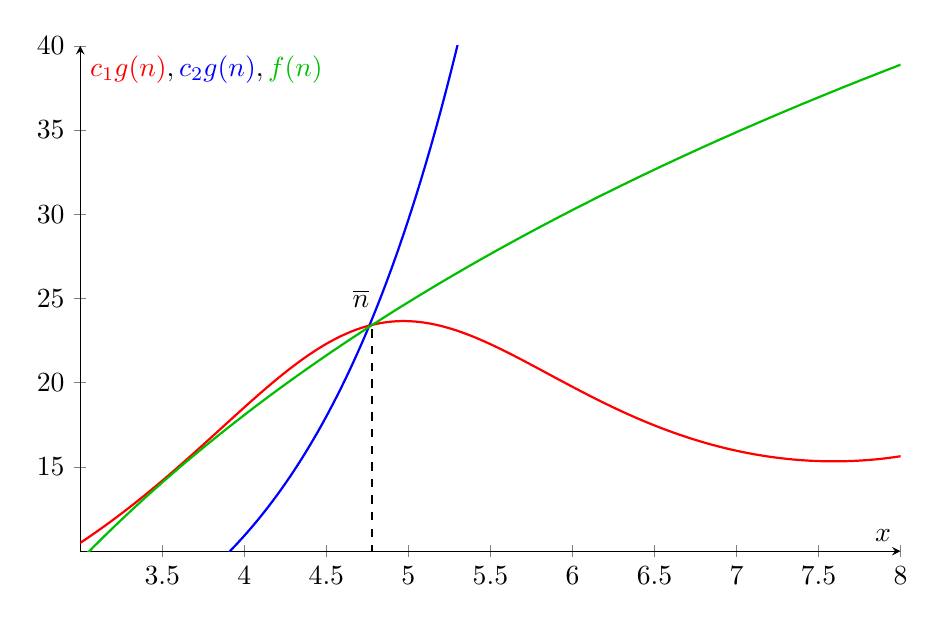
\begin{tikzpicture}
    \begin{axis}[
        axis lines = middle,
        xlabel = $x$,
        ylabel = {$\textcolor{red}{c_1g(n)}, \textcolor{blue}{c_2g(n)}, \textcolor{green!75!black}{f(n)}$},
        legend pos=north west,
        domain=2:8,
        samples=200,
        xmin=3, xmax=8, ymin=10, ymax=40,
        width=12cm,
        height=8cm
    ]
        \addplot[color=blue, thick] {(exp(x))/5};
        \addplot[color=red, thick] {(30*ln(x))/(sin(deg(x)) + 3)};
        \addplot[color=green!75!black, thick] {30*ln(x) - 23.5};


        % Add a vertical line at the intersection point
        \addplot[mark=none, black, dashed, thick] coordinates {(4.78, 0) (4.78, 23.65)};
        \node at (axis cs:4.6,25) [anchor=west] {$\overline{n}$};

    \end{axis}
\end{tikzpicture}
\end{figure}



\begin{examplebox}{Esempio 1}
Questa affermazione vale?
\[n \in O(2n)\]
Sì, perché esiste un $c$ che soddisfa $n \le c2n$.\\\\
Quest'altra affermazione vale?
\[2n \in O(n)\]
Sì perché esiste un $c$ che soddisfa $2n \le 2n$.
\end{examplebox}
\begin{examplebox}{Esempio 2}
Questa affermazione vale?
\[f \in O(g) \Longleftrightarrow g \in \Omega(g)\]
Proviamo a dimostrare. Sappiamo che esiste un $c$ e $\overline{n}$ tale che \(\forall n > \overline{n} \; f(n) \le cg(n)\). Isoliamo la g:
\[g(n) \ge \frac{1}{c} f(n)\]
Esiste quindi un c' che soddisfa la disuguaglianza.
\[c' = \frac{1}{c}\]
\end{examplebox}
\begin{examplebox}{Esempio 3}

\[f_1 \in O(g),
f_2 \in O(g) \Longrightarrow f_1 + f_2 \in O(g)
\]
Dobbiamo dimostrare che esiste $c_1$ e $c_2$, $\overline{n}_1$ e $\overline{n}_2$ tali che:
\[\forall n > \overline{n}_1 \; | \; f_1(n) \le c_1g(n)\]
\[\forall n > \overline{n}_2 \; | \; f_2(n) \le c_2g(n)\]
Quindi
\[\overline{n} = max(\overline{n}_1, \overline{n}_2)\]
\[f_1(n) + f_2(n) \le (c_1 + c_2)g(n)\]

\end{examplebox}

\begin{examplebox}{Esempio 4}
    \[f_1 \in O(g_1), f_2 \in O(g_2) \; | \; f_1f_2 \in O(g_1g_2)\]
Quindi esiste $c_1$ e $c_2$, $\overline{n}_1$ e $\overline{n}_2$ tali che:
\[\forall n > \overline{n}_1 \; | \; f_1(n) \le c_1g(n)\]
\[\forall n > \overline{n}_2 \; | \; f_2(n) \le c_2g(n)\]
\[f_1(n)f_2(n) \le c_1g_1(n)c_2g_2(n)\]
\[f_1(n)f_2(n) \le c_1c_2g_1(n)g_2(n)\]
Quindi:
 \[c = c_1c_2\] \[\overline{n} = max(\overline{n}_1, \overline{n}_2)\]
\end{examplebox}

\subsection{Ordini di grandezza per le funzioni}

L'algoritmo di ricerca $A$ termina entro n. Immaginiamo che l'algoritmo A sia il seguente:
\begin{lstlisting}
For i <- 0 to length(a) - 1
    if a[i] = x
        ret i
ret -1
\end{lstlisting}
Capiamo che la sua complessità è uguale a:
\[A \in O(n)\]
Per appurarci che la stima di complessità sia accurata dobbiamo controllare che $A \in \Omega(g)$ vuol dire che esiste uno schema di input tale per cui se $g(n)$ è il numero di passi necessari per risolvere l'istanza $n$, allora $g \in \Omega(f)$. Se riusciamo a fare questo allora $g \in \Theta(f)$ e quindi possiamo dire che la stima è accurata.
\\\\
$P \in O(f)$ vuol dire che il problema $P$ riesco a risolvere in tempo $f$. Supponiamo per assurdo che esista un algoritmo riesca a capire se l'elemento si trova nell'array o no. Possiamo capire velocemente che per contraddizione, essendo che esiste almeno un elemento dove l'algoritmo non ha guardato, siamo certi del malfunzionamento dell'algoritmo e quindi non è vero che esiste una stima di complessità più bassa di $f$.


Ora andiamo ad affrontare i tipi di algoritmi che si definiscono di "ordinamento".
\begin{definition}
\textbf{Input}: Sequenza $(a_1, ..., a_n)$ di oggetti su cui è definita una relazione di ordinamento (in questo caso ordinamento per confronti).
\\\\
\textbf{Output}: Permutazione $(a_1', ..., a_n')$ di $(a_1, ..., a_n)$ t.c. $\forall \, i > j, \; \; a_i' \le a_j'$.
\end{definition}
Andiamo ora a vedere i diversi tipi di algoritmi di ordinamento.

\subsection{insertion$\_$sort (A)}

In questo caso la $j$ sarà chiamata variabile "invariante" ovvero che mantiene una proprietà che continua a valere nel run-time dell'algoritmo. In questo caso, la $j$ è invariante perchè tutti gli oggetti "a sinistra" di essa saranno considerati già ordinati. (Parte da 2 perché abbiamo deciso che la posizione all'interno dell'array parte da 1).

\begin{lstlisting}
for j <- 2 to length[A]
    key <- A[j]
    i <- j - 1
    while i > 0 and A[i] > key
        A[i+1] <- A[i]
        i--
    a[i+1] <- key
\end{lstlisting}
Ora dobbiamo capire quale sia la complessità di questo algoritmo. Se le cose vanno bene, l'algoritmo potrebbe terminare in $O(n)$. Tuttavia, seppur giusto, non è preciso. Infatti, nel peggiore dei casi, l'algoritmo termina in $O(n^2)$. Infatti il caso peggiore di input che mi può arrivare è un array ordinato al contrario con complessità uguale a:
\[1 + 2 + 3 + ... + n = \frac{n(n+1)}{2} \in \Theta(n^2)\]
\textit{Questo algoritmo, quanto spazio di memoria usa in più rispetto allo spazio occupato dai dati? }
\\\\
Lo spazio di memoria di questo algoritmo rimane costante a prescindere dalla dimensione del problema. Un algoritmo del genere si dice che \textit{\textbf{ordina in loco}} se la quantità di memoria extra è costante. Si parla di \textit{\textbf{stabilità}} di un algoritmo di ordinamento quando l'ordine relativo di elementi uguali non viene scambiato dall'algoritmo. Quindi:
\[\text{Se } a_i = a_j \, i < j, \text{mantiene l'ordinamento}\]


\section{Concetto di "Divide et impera"}

\subsection{Fattoriale e funzioni ricorsive}

\begin{lstlisting}
Fatt(n)
    if n = 0
        ret 1
    else
        ret n * fatt(n - 1)
\end{lstlisting}

L'argomento della funzione ci fa capire la complessità dell'algoritmo:
\[
  T(n) = \begin{cases}
    1 & \text{se } n = 0 \\
    T(n - 1) + 1 & \text{se } n > 0
  \end{cases}
\]
Con problemi ricorsivi si avrà una complessità con funzioni definite ricorsivamente.
Questo si risolve induttivamente:
\[
  \begin{aligned}
    T(n) & = 1 + T(n-1)\\
         & = 1 + 1 + T(n-2)\\
         & = 1 + 1 + 1 + T(n-3)\\
         & = \underbrace{1 + 1 + \ldots + 1}_{i} + T(n-i)\\
  \end{aligned}
\]
La condizione di uscita è: \( n-i = 0 \quad n = i \)
\[
\begin{aligned}
         & = \underbrace{1 + 1 + \ldots + 1}_{n} + T(n-n)\\
         & = n + 1 = \Theta(n)
\end{aligned}
\]
Questo si chiama passaggio iterativo.

\begin{examplebox}{Esempio 1}
  \[
    T(n) = 2T\left(\floor*{\frac{n}{2}}\right) + n
  \]
  Questa funzione si può riscrivere come:
  \[
  T(n) = \begin{cases}
    \text{Costante} & \text{se } n < a \\
    2T\left(\floor*{\frac{n}{2}}\right) + n & \text{se } n \ge a
  \end{cases}
  \]

  \vspace{1em}
  \noindent
  Se la complessità fosse già data bisognerebbe soltanto verificare se è corretta.
  Usando il metodo di sostituzione:
  \[
    T(n) = cn \log n
  \]
  sostituiamo nella funzione di partenza:
  \[
    \begin{aligned}
      T(n)  & = 2T\left(\floor*{\frac{n}{2}}\right) + n\\
            & \le 2c\left(\floor*{\frac{n}{2}}\right) \log \floor*{\frac{n}{2}} + n\\
            & \le \cancel{2} c \frac{n}{\cancel{2}} \log \frac{n}{2} + n\\
            & = cn \log n - cn \log 2 + n\\
            & \stackrel{?}{\le} cn \log n \quad \text{se } n- cn \log 2 \le 0\\
    \end{aligned}
  \]
  \[
    c \ge \frac{n}{n \log 2} = \frac{1}{\log 2}
  \]
  Il metodo di sostituzione dice che quando si arriva ad avere una disequazione
  corrispondente all'ipotesi, allora la soluzione è corretta se soddisfa una certa ipotesi.
\end{examplebox}

\begin{examplebox}{Esempio 2}
  \[
    T(n) = T\left(\floor*{\frac{n}{2}}\right) + T\left(\ceil*{\frac{n}{2}}\right) + 1 \quad \in O(n)
  \]
  \[
  T(n) \le cn
  \]
  \[
  \begin{aligned}
    T(n) & = T\left(\floor*{\frac{n}{2}}\right) + T\left(\ceil*{\frac{n}{2}}\right) + 1\\
         & \le c\left(\floor*{\frac{n}{2}}\right) + c\left(\ceil*{\frac{n}{2}}\right) + 1\\
         & = c \left( \left\lfloor \frac{n}{2} \right\rfloor + \left\lceil \frac{n}{2} \right\rceil  \right) + 1\\
         & = cn + 1 \stackrel{?}{\le} cn
  \end{aligned}
  \]
  Il metodo utilizzato non funziona perchè rimane l'1 e non si può togliere in alcun modo.
  Per risolvere questo problema bisogna risolverne uno più forte:
  \[
  T(n) \le cn - b
  \]
  \[
  \begin{aligned}
    T(n) & = T\left(\floor*{\frac{n}{2}}\right) + T\left(\ceil*{\frac{n}{2}}\right) + 1\\
         & \le c\left(\floor*{\frac{n}{2}}\right) -b + c\left(\ceil*{\frac{n}{2}}\right) -b + 1\\
         & = c \left( \left\lfloor \frac{n}{2} \right\rfloor + \left\lceil \frac{n}{2} \right\rceil  \right) - 2b + 1\\
         & = cn - 2b + 1 \stackrel{?}{\le} cn - b\\
         & = \underbrace{cn - b} + \underbrace{1 - b}_{\le 0} \le cn - b \quad \text{se } b \ge 1\\
  \end{aligned}
  \]
  Se la proprietà vale per questo problema allora vale anche per il problema iniziale
  perchè è meno forte.
\end{examplebox}

\begin{examplebox}{Esempio 3}
  \[
    \begin{aligned}
      T(n) & = 3T \left( \left\lfloor \frac{n}{4} \right\rfloor \right) + n\\
           & = n + 3T \left( \left\lfloor \frac{n}{4} \right\rfloor \right)\\
           & = n + 3 \left( \left\lfloor \frac{n}{4} \right\rfloor + 3T
           \left( \left\lfloor \frac{\left\lfloor \frac{n}{4} \right\rfloor}{4} \right\rfloor
           \right)  \right)\\
           & = n + 3 \left\lfloor \frac{n}{4} \right\rfloor + 3^2 T
           \left( \left\lfloor \frac{n}{4^2} \right\rfloor \right)\\
           & \le n + 3 \left\lfloor \frac{n}{4} \right\rfloor + 3^2
           \left( \left\lfloor \frac{n}{4^2} \right\rfloor + 3T \left(
           \left\lfloor \frac{\left\lfloor \frac{n}{4^2} \right\rfloor}{4} \right\rfloor
           \right)  \right) \\
           & = n + 3 \left\lfloor \frac{n}{4} \right\rfloor + 3^2
           \left\lfloor \frac{n}{4^2} \right\rfloor + 3^3 T
           \left( \left\lfloor \frac{n}{4^3} \right\rfloor \right) \\
           & = n + 3 \left\lfloor \frac{n}{4} \right\rfloor + \ldots + 3^{i-1}
           \left\lfloor \frac{n}{4^{i-1}} \right\rfloor + 3^i T
           \left( \left\lfloor \frac{n}{4^i} \right\rfloor \right)
    \end{aligned}
  \]


  Per trovare il caso base poniamo l'argomento di T molto piccolo:
  \[
    \begin{aligned}
      \frac{n}{4^i} & < 1\\
      4^i & > n\\
      i & > \log_4 n
    \end{aligned}
  \]
  L'equazione diventa:
  \[
    \begin{aligned}
      & \le n + 3 \left\lfloor \frac{n}{4} \right\rfloor + \ldots + 3^{\log_4 n - 1}
      \left\lfloor \frac{n}{4^{\log_4 n - 1}} \right\rfloor + 3^{\log_4 n} c\\
    \end{aligned}
  \]


  Si può togliere l'approssimazione per difetto per ottenere un maggiorante:
  \[
  \begin{aligned}
    & \le n \left( 1 + \frac{3}{4} + \left( \frac{3}{4} \right)^2 + \ldots +
    \left( \frac{3}{4} \right)^{\log_4 n-1} \right) + 3^{\log_4 n} c\\
    & \le n \left( \sum_{i=0}^{\infty} \left( \frac{3}{4} \right)^i \right) + c 3^{\log_4 n}\\
  \end{aligned}
  \]
  Per capire l'ordine di grandezza di \( 3^{\log_4 n} \) si può scrivere come:
  \[
    3^{\log_4 n} = n^{\left( \log_n 3^{\log_4 n} \right) } = n^{\log_4 n \cdot \log_n 3}
    = n^{\log_4 3}
  \]
  Quindi la complessità è:
  \[
  \begin{aligned}
    & = O(n) + O(n^{\log_4 3})\\
  \end{aligned}
  \]
  Si ha che una funzione è uguale al termine noto della funzione originale e l'altra
  che è uguale al logaritmo dei termini noti. Se usassimo delle variabili uscirebbe:
  \[
    \begin{aligned}
      T(n) & = a T \left( \left\lfloor \frac{n}{b} \right\rfloor \right) + f(n)\\
           & = O(f(n)) + O(n^{\log_b a})
    \end{aligned}
  \]
\end{examplebox}



\subsection{Master Theorem o Teorema dell'esperto}

Data una relazione di occorrenza di questa forma:

\[T(n) = a T \left( \left\lfloor \frac{n}{b} \right\rfloor \right) + f(n)\]

Distinguiamo tre casi:

\begin{enumerate}
    \item \[f(n) \in O(n^{\log_ba - \epsilon}) \Longrightarrow T(n) \in \Theta(n^{\log_ba})\]
    \item \[f(n) \in \Theta(n^{\log_ba}) \Longrightarrow T(n) \in \Theta(f(n)\log n)\]
    \item \[f(n) \in \Omega(n^{\log_ba + \epsilon} ) \Longrightarrow T(n) \in \Theta(f(n))\]
\end{enumerate}

\begin{examplebox}{Esempio 1}
    \[T(n) = 9T\left(\frac{n}{3}\right) + n\]
    \[a = 3, b = 3, f(n) = n\]
    Basta che trovo un $\epsilon$ che mi dia $n$.
    \[n^{\log_b a} = n^{\log_3 9} = n^2 * n^{-\frac{1}{2}}\]
    In questo caso $\epsilon = n^{-\frac{1}{2}}$ e ci troviamo nel \textbf{PRIMO CASO} e la soluzione è $T(n) \in \Theta(n^2)$.
\end{examplebox}

\begin{examplebox}{Esempio 2}
       \[T(n) = T\left(\frac{2n}{3}\right) + 1\]
    \[a = 1, b = \frac{3}{2}, f(n) = n^0\]
    \[n^{\log_b a} = n^{\log_{\frac{3}{2}} 1} = n^0\]
    Ci troviamo nel \textbf{SECONDO CASO} e la soluzione è $T(n) \in \Theta(\log n))$
\end{examplebox}

\begin{examplebox}{Esempio 3}
    \[T(n) = 3T\left(\frac{n}{4}\right) + n \log n\]
       \[a = 3, b = 4, f(n) = n \log n\]
       Ci troviamo nel \textbf{TERZO CASO} quindi basta qualsiasi valore di $\epsilon$ basta che sia contenuto tra $\log_3 4 \le \epsilon \le 1$. La soluzione è $T(n) \in \Theta(n\log n)$.
\end{examplebox}

\begin{examplebox}{Esempio 4}
    \[T(n) = 2T\left(\frac{n}{2}\right) + n \log n\]
       \[a = 2, b = 2, f(n) = n \log n\]
    \[n\log n \in \Omega(n^{1 + \stackrel{?}{\epsilon}}) \]
    \[\log n \in \Omega(n^\epsilon) \text{ NON VALE}\]
    Poiché un logaritmo è sempre più piccolo di un polinomio.
    Questo è un caso dove il teorema \textit{non} si applica
\end{examplebox}


\subsection{Merge Sort (A, n)}

Questo algoritmo di ordinamento \textit{ricorsivo} utilizza il concetto di \textit{divide et impera}.

Concettualmente, un merge sort funziona come segue:

\begin{enumerate}
    \item \textbf{Dividi} l'array non ordinato in n sottoarray, ognuno contenente un elemento (un array di un elemento è considerato ordinato).
    \item \textbf{Unisci} ripetutamente i sottoarray per produrre nuovi sottoarray ordinati finché non ne rimane solo uno. Questo sarà l'array ordinato.
\end{enumerate}
La sua complessità considerando il merge con complessità lineare risulta:
\[T(n) = 2T\left(\frac{n}{2}\right) + n\]
Utilizzando il \textbf{Master Theorem} e cadendo del \textit{secondo caso} possiamo confermare che il risultato è:
\[= \Theta(n \log n)\]

\begin{lstlisting}[language=Scala]
// A e' l'array mentre p ed r sono rispettivamente l'indice di partenza e di arrivo
mergeSort(A, p, r) // O(n log n)
    if (p < r)
        q <- floor((p+r)/2)
        mergeSort(A, p, q)
        mergeSort(A, q+1, r)
        merge(A, p, q, r)
\end{lstlisting}
\begin{lstlisting}[language=Scala]
merge(A, p, q, r)
    i <- 1
    j <- p
    k <- q+1
    // Ordina gli elementi di A in B
    // O il lato sinistro ha finito
    while(j <= q or k <= r) // O(n)
        if j <= q and (k > r or A[j] <= A[k])
            B[i] <- A[j]
            j++
        else
            B[i] <- A[k]
            k++
        i++
    // Copia gli elementi di B in A
    for i <- 1 to r-p+1  // O(n)
        A[p+i-1] <- B[i]
\end{lstlisting}
L'algoritmo è \textbf{stabile} poiché non vengono scambiati gli elementi uguali. Tuttavia non ordina \textbf{in loco} poiché utilizza uno spazio di memoria aggiuntivo.
\subsection{Heap}
L'Heap è un albero semicompleto (ogni nodo ha 2 figli ad ogni livello tranne l'ultimo  che è completo solo fino ad un certo unto) in cui i nodi contengono oggetti con relazione di ordinamento.\\\\
\textbf{\textit{Proprietà Heap:}}

\[\forall \text{ nodo, il contenuto è } \ge \text{ del contenuto dei figli}\]

\begin{figure}[H]
    \centering

    \begin{forest}
for tree={
    draw, % Disegna i nodi
    circle, % Forma dei nodi
    minimum size=1.5em, % Dimensione minima dei nodi
    inner sep=1pt, % Spaziatura interna dei nodi
    s sep=1.5cm % Spaziatura verticale tra i livelli
}
  [16, edge label={node[right, xshift=7pt] {1}}
    [14, edge label={node[above, yshift=7pt] {2}}
      [8, edge label={node[above, yshift=7pt] {4}}
        [1, edge label={node[above, yshift=7pt] {8}}]
        [2, edge label={node[above, yshift=7pt] {9}}]
      ]
      [9, edge label={node[above, yshift=7pt] {5}}
        [3, edge label={node[right, xshift=7pt] {10}}]
      ]
    ]
    [10, edge label={node[above, yshift=7pt] {3}}
      [2, edge label={node[above, yshift=7pt] {6}}]
      [3, edge label={node[above, yshift=7pt] {7}}]
    ]
  ]
\end{forest}
    \label{fig:enter-label}
\end{figure}
La complessità dell'algoritmo è in base al numero di livelli dell'albero.\\\\
$\longrightarrow$ albero con $n$ livelli:
\[\# \text{Nodi} = 2^0 + 2^1 + 2^2 + ... + 2^{n - 1} = \frac{1 - 2^n}{1-2} = 2^n - 1\]
$\longrightarrow$ albero con $n$ nodi:
\[\# \text{Livelli} = \log_2n\]
\[\#\text{Foglie} = \frac{n}{2}\]
Le foglie di un albero sono la metà dei nodi dell'albero.

\begin{lstlisting}[language=Scala]
extractMax(H) // O(log n)
    h[1] <- H[H.heap_size()]
    H.heap_size()--
    heapify(H, 1)
\end{lstlisting}

\begin{lstlisting}[language=Scala]
heapify(H, 1) // O(log n)
    l <- left[i] //
    r <- right[i]
    if(l < h.heap_size() AND H[l] > H[i]
        largest <- l
    else
        largest <- i
    if m <= h.heap_size() and H[r] > H[largest]
        largest <- r
    if largest != i
        swap(H[i], H[largest])
        heapify(H, largest)
\end{lstlisting}
Creare uno heap da un array:
\begin{lstlisting}[language=Scala]
buildHeap(A)
    A.heap_size() <- length[A]
        for i <- length[A]/2 down to 1
            heapify(A, i)
\end{lstlisting}
Immagino tutte le foglie come heap con un solo nodo. L'indice del primo nodo che non è heap corrisponde a $\frac{length(A)}{2}$ su questo allora chiamo \texttt{heapify}.

\pagebreak

\subsection{Heapsort}
\begin{lstlisting}[language=Scala]
HeapSort(A) // O(n log n)
    buildHeap(A)
    for i <- length(A) to 1
        scambia(A[1], A[i])
        heapsize(A)--
        heapify(a, i)
\end{lstlisting}
L'Heap Sort è un algoritmo che lavora \textbf{in loco} tuttavia non è \textbf{stabile}. Tuttavia riusciamo a fare una stima migliore e più corretta?
\[n \log i = \sum_{i=1}^n \log i = \log \prod_{i=1}^n i = \log n! = \Theta(\log n^n) = \Theta(n \log n)\]
In questo caso, essere accurati non aiuta, ma abbiamo avuto la certezza che non esiste una stima migliore.
\subsection{Quicksort}
Come funziona l'algoritmo?
\begin{enumerate}
    \item Dividi prima l'array in due parti. (Partizione)
    \item  Devi essere sicuro che tutti gli elementi di sinistra siano $\le$ di quelli di destra. Ricorsivamente ordina la parte sinistra e la parte destra.
    \item A questo punto l'array è ordinato.
\end{enumerate}

\begin{lstlisting}[language=Scala]
quickSort(A, p, r)
    if (p < r)
        q <- partition(a, p, r)
        quickSort(A, p, q)
        quickSort(A, q+1, r)
\end{lstlisting}

\begin{lstlisting}[language=Scala]
partition(A, p, r) // O(n)
    x <- A[p] // Elemento Perno
    i <- p-1
    k <- r+1
    while true
        repeat j-- until a[j] <= x
        repeat i++ until a[i] >= x
        if i < j
            scambia(a[i], a[j])
        else
            ret j
\end{lstlisting}
Scegliamo un elemento a caso in base a quello comparato rispetto all'elemento perno tale che:
\[sx \le perno \le dx\]
Questo algoritmo non è \textbf{stabile} ma lavora \textbf{in loco}.
La sua complessità?
\[T(n) = T(\text{partition}) + T(q) + T(n-q)\]
Se il quicksort è perfettamente diviso in due, allora la sua complessità è $O(n \log n)$.
Se invece l'array è già ordinato la sua equazione di ricorrenza sarà:
\[= n + T(1) + T(n-1) = \colorbox{yellow!50!white}{$\Theta(n^2)$}\]
Tuttavia non ci aspettiamo che questo caso sia frequente e quindin nella stra grande maggioranza dei casi allora:
\[T(n) = n + T(cn) + T((1-c)n)\]
Un equazione di questo tipo sappiamo che ha come complessità $\Theta(n \log n)$.
\begin{lstlisting}[language=Scala]
rand_Partition(A, p, r)
    i <- rand(p .. r) // Ora l'elemento perno e' un elemento a caso
    scambio(A[p], A[i]
    ret partition(A, p, r)
\end{lstlisting}

\begin{align*}
    T(n) &= n + \frac{1}{n}(T(1) + T(n-1) + \frac{1}{n}(T(2) + (T-2)) + \; \dots \; + \\
    & \frac{1}{n}(T(n-2) + T(2)) + \frac{1}{n}(T(n-1) + T(1) = \\
    &= n + \frac{1}{n} \sum_{i}(T(i) + T(n-i))\\
    &= n + \frac{2}{n} \sum_{i} T(i) \in \colorbox{green!30!white}{$O(n \log n$)}
\end{align*}
Qualsiasi algoritmo che\textit{ lavora per confronti }deve fare almeno $O(n \log n)$.

\section{Algoritmi di ordinamento in tempo lineare}

\subsection{Algoritmi non basati su confronti}

\subsubsection{Counting Sort}
Tuttavia possiamo trovare algoritmi che come tempo
di esecuzione hanno tempo lineare. Come?
Non lavorando a \textbf{confronti}.
\\\\
Come ordinare $n$ numeri con valori da 1 a $k$?
\begin{lstlisting}[language=Scala]
countingSort(A, k)
    for i <- 1 to k
        C[i] <- 0
    for j <- 1 to len(A)
        C[A[j]]++
    for i <- 2 to k
        C[i] <- C[i-1]+C[i]
    for j <- len(A) down to 1
        B[C[A[j]]] <- a[j]
        C[A[J]]--
\end{lstlisting}
La complessità di questo algoritmo è $O(n + k)$ dove $n$ è la lunghezza dell'array e $k$ e il range di valori.

\subsubsection{Radix Sort}

Il radix sort è un algoritmo di ordinamento che ordina gli elementi
confrontando i singoli bit. Quello che fa è ordinare per la cifra meno
significativa, poi per la seconda cifra meno significativa e così via.


\begin{lstlisting}[language=Scala]
radixSort(A, d) // O(d(n+k))
  for i <- 1 to d
      countingSort(A, n)
\end{lstlisting}
La complessità di questo algoritmo è \[\Theta(d(n+k))\]dove $d$ è il numero di cifre e $k$ è il range di valori.
Se si vuole invece ordinare $n$ valori da 1 a $n^2 - 1$, le costanti nascoste all'interno
del $\Theta$ sono molto alte e quindi non è un algoritmo efficiente. Tuttavia
si posson rappresentare i numeri in base $n$ e quindi ottenere un algoritmo lineare.

\subsubsection{Bucket Sort}

Il Bucket Sort è un algoritmo di ordinamento che funziona bene quando i dati sono distribuiti uniformemente. Quindi
su un array di $n$ elementi \textbf{distribuiti uniformemente} su $[0, 1)$, si può dividere l'intervallo in $n$ sottointervalli
con probabilità $\frac{1}{n}$ e poi ordinare i singoli sottointervalli chiamate anche \textit{"Bucket"}.
Infatti se i dati sono distribuiti uniformemente allora la complessità dell'algoritmo è lineare: \[\Theta(n)\]Questo
perché in ogni bucket ci si aspetta un valore costante e quindi indipendente dal valore di $n$.
\\\\Il caso pessimo però è quando tutti gli elementi ricadono nello stesso bucket. La probabilità che questo accada è molto bassa
infatti è: \[\underbrace{\frac{1}{n} \ast \frac{1}{n} \ast \dots \ast \frac{1}{n}}_{n-1}  = \frac{1}{n^{n-1}}\]e la sua complessità diventa: \[O(n^2)\]
\\\\
Sia \(X_{ij}\) la variabile aleatoria che vale:
\[
\begin{cases}
  1 & \text{Se l'elemento } i \text{ va nel bucket } j\\
  0 & \text{altrimenti}
\end{cases}
\]
Per esprimere il numero di elementi nel bucket $j$ si ha:
\[
  N_j = \sum_{i} X_{ij}
\]
La complessità di questo algoritmo quindi può essere espressa come:
\[
  C = \sum_j {N_j}^2
\]
Dove il valore atteso è:
\[E[C] = E\left[ \sum_j {N_j}^2\right] = \sum_j E[{N_j}^2] = \sum_j\left(Var(N_j) - E[N_j]^2\right)\]
Dove $E[N_j]$ è:
\[E[N_j] = \sum E[X_{ij}] = \sum_{j=1}^n \frac{1}{n} = 1\]
\[Var[N_j] = \sum Var(X_{ij}) = \sum \frac{1}{n} * \left(1 - \frac{1}{n}\right) = 1 - \frac{1}{n}\]
E quindi possiamo svolgere il calcolo precedente dove:

\begin{align*}
  \sum_j \left(Var(N_j) - E[N_j]^2\right) &=  \sum_j \left(\left(1 - \frac{1}{n}\right) + 1\right) \\ &= \sum_j 2 - \frac{1}{n}\\  &= 2n - 1
\end{align*}
Le distribuzioni possono essere arbitrarie ma basta che tutti i bucket abbiano la stessa probabilità.
Prendiamo:
\[n_1, ..., n_2, ... , n_l\]
\[\frac{1}{n_1}, \, ... \,  , \frac{1}{n_2}, \, ... \, , \frac{1}{n_l}\]
La \textit{turing-riduzione} è un algoritmo che riduce un problema ad un altro problema.


\section{Algoritmi di selezione}
Dato in input un array \( A \) di oggetti su cui è definita una relazione di ordinamento
e un indice \( i \) compreso tra \( 1 \) e \( n \) (\( n \) è il numero di oggetti
nell'array), l'output dell'algoritmo è l'oggetto che si trova in posizione \( i \)
nell'array ordinato.
\begin{lstlisting}[language=Scala]
selezione(A, i)
  ordina(A) // O(n log n)
  return A[i]
\end{lstlisting}
Quindi la complessità di questo algoritmo nel caso peggiore è \( O(n \log n) \)
(limite superiore). È possibile selezionare un elemento in tempo lineare? Analizziamo
un caso particolare dell'algoritmo di selezione, ovvero la ricerca del minimo (o del massimo).


\subsection{Ricerca del minimo o del massimo}
\vspace{1em}
\noindent
In tempo lineare si può trovare il minimo e il massimo
di un array:
\begin{lstlisting}[language=Scala]
minimo(A)
  min <- A[1]
  for i <- 2 to length[A]
    if A[i] < min
      min <- A[i]
  return min
\end{lstlisting}
trovare il minimo equivale a trovare \texttt{selezione(A, 1)} e trovare il massimo
equivale a trovare \texttt{selezione(A, n)}. Si può però andare sotto la complessità
lineare?

\vspace{1em}
\noindent
Per trovare il massimo (o il minimo) elemento \( n \) di un array bisogna fare
\textbf{almeno} \( n-1 \) confronti perchè bisogna confrontare ogni elemento con
l'elemento massimo (o minimo) trovato per poter dire se è il massimo (o minimo).
Di conseguenza, non è possibile avere un algoritmo per la ricerca del massimo (o minimo)
in cui c'è un elemento che non "perde" mai ai confronti (cioè risulta sempre il più
grande) e non viene dichiarato essere il più grande (o più piccolo).

\vspace{1em}
\noindent
\textbf{Dimostrazione}:
Per dimostrarlo si può prendere un array in cui l'elemento \( a \) non perde mai ai
confronti, ma l'algoritmo dichiara che il massimo è l'elemento \( b \). Allora si rilancia
l'algoritmo sostituendo l'elemento \( a \) con \( a = \text{\texttt{max(b+1,a)}} \) e si
ripete l'algoritmo con questo secondo array in cui \( a \) è l'elemento più grande. Si ha
quindi che i confronti in cui \( a \) non è coinvolto rimangono gli stessi e i confronti
in cui \( a \) è coinvolto non cambiano perchè anche prima \( a \) non perdeva mai ai
confronti, di conseguenza l'algoritmo dichiarerà che il massimo è \( b \) e quindi
l'algoritmo non è corretto, dimostrando che non esiste un algoritmo che trova il massimo
in meno di \( n-1 \) confronti.

\vspace{1em}
\noindent
Abbiamo quindi trovato che la complessità del massimo (o minimo) nel caso migliore è
\( \Omega(n) \) (limite inferiore) e nel caso peggiore è \( O(n) \) (limite superiore).
Di conseguenza la complessità è \( \Theta(n) \).

\subsubsection{Ricerca del minimo e del massimo contemporaneamente}
Si potrebbe implementare unendo i 2 algoritmi precedenti:
\begin{lstlisting}[language=Scala]
min_max(A)
  min <- A[1]
  max <- A[1]
  for i <- 2 to length[A]
    if A[i] < min
      min <- A[i]
    if A[i] > max
      max <- A[i]
  return (min, max)
\end{lstlisting}
Questo algoritmo esegue \( n-1 + n-1 = 2n-2 \) confronti.

\begin{itemize}
  \item \textbf{Limite inferiore}: Potenzialmente ogni oggetto potrebbe essere il minimo
    o il massimo. Sia \( m \) il numero di oggetti potenzialmente minimi e \( M \) il
    numero di oggetti potenzialmente massimi. Sia \( n \) il numero di oggetti nell'array.
    \begin{itemize}
      \item All'inizio \( m+M = 2n \) perchè ogni oggetto può essere sia minimo che
        massimo.
      \item Alla fine \( m+M = 2 \) perchè alla fine ci sarà un solo minimo e un solo
        massimo.
    \end{itemize}
    Quando viene fatto un confronto \( m+M \) può diminuire.
    \begin{itemize}
      \item Se si confrontano due oggetti che sono potenzialmente sia minimi che massimi,
        allora \( m+M \) diminuisce di \( 2 \) perchè:
        \[
          a < b
        \]
        \( b \) non può essere il minimo e \( a \) non può essere il massimo e si perdono
        2 potenzialità.

      \item Se si confrontano due potenziali minimi (o massimi), allora \( m+M \)
        diminuisce di \( 1 \) perchè:
        \[
          a < b
        \]
        \( b \) non può essere il minimo e si perde 1 potenzialità.
    \end{itemize}
    Un buon algoritmo dovrebbe scegliere di confrontare sempre 2 oggetti che sono
    entrambi potenziali minimi o potenziali massimi.

    \vspace{1em}
    \noindent
    Due oggetti che sono potenzialmente sia minimi che massimi esistono
    se \( m+M > n+1 \) perchè se bisogna distribuire n potenzialità ne avanzano
    due che devono essere assegnate a due oggetti che hanno già una potenzialità.
    Quindi fino a quando \( m+M \) continua ad essere almeno \( n+2 \) si riesce a
    far diminuire \( m+M \) di 2 ad ogni confronto.

    Questa diminuzione si può fare \( \left\lfloor \frac{n}{2} \right\rfloor \) volte,
    successivamente \( m+M \) potrà calare solo di 1 ad ogni confronto.

    \vspace{1em}
    \noindent
    Successivamente il numero di oggetti rimane:
    \[
      \begin{cases}
        n+1 & \text{se } n \text{ è dispari}\\
        n & \text{se } n \text{ è pari}
      \end{cases}
    \]
    \begin{itemize}
      \item \( n \) dispari:
        \[
          \begin{aligned}
            &n+1 - 2 + \left\lfloor \frac{n}{2} \right\rfloor\\
            &= n-1 + \left\lfloor \frac{n}{2} \right\rfloor\\
            &= \left\lfloor \frac{3}{2}n \right\rfloor - 1\\
            &= \left\lceil \frac{3}{2}n \right\rceil - 2\\
          \end{aligned}
        \]

      \item \( n \) pari:
        \[
          \begin{aligned}
            &n - 2 + \left\lfloor \frac{n}{2} \right\rfloor \\
            &= n-2 + \frac{n}{2}\\
            &= \frac{3}{2}n - 2\\
            &= \left\lceil \frac{3}{2}n \right\rceil -2
          \end{aligned}
        \]
    \end{itemize}
    Quindi la complessità è \( \Omega(\left\lceil \frac{3}{2}n \right\rceil -2) = \Omega(n)
    \) (limite inferiore). Meglio di così non si può fare, ma non è detto che esista
    un algoritmo che raggiunga questo limite inferiore.
\end{itemize}
Un algoritmo che raggiunge il limite inferiore è il seguente:
\begin{enumerate}
  \item Dividi gli oggetti in 2 gruppi:
    \[
      \underbrace{
        \underbrace{
          \begin{aligned}
          &a_1\\
          &a_2\\
          &\vdots\\
          &a_{\left\lfloor \frac{n}{2} \right\rfloor}
          \end{aligned}
        }_{\text{Potenziali minimi}}
        \quad
        \underbrace{
          \begin{aligned}
        &b_1\\
        &b_2\\
        &\vdots\\
        &b_{\left\lceil \frac{n}{2} \right\rceil}
          \end{aligned}
        }_{\text{Potenziali massimi}}
      }_{\text{Potenziali sia minimi che massimi}}
    \]

  \item Confronta \( a_i \) con \( b_i \), supponendo \( a_i < b_i \) (mette a sinistra
    i più piccoli e a destra i più grandi). Una volta aver fatto il confronto possiamo swappare
     gli elementi nella loro apposita sezione.

  \item Cerca il minimo degli \( a_i \) e cerca il massimo dei \( b_i \):

  \item Sistema l'eventuale elemento in più (se l'array è dispari)
\end{enumerate}

\subsection{Randomized select}
Si può implementare un algoritmo che divide l'array in 2 parti allo stesso modo
in cui viene effettuata la \texttt{partition} di quick sort:
\begin{lstlisting}[language=Scala]
// A: Array
// p: Indice di partenza
// r: Indice di arrivo
// i: Indice che stiamo cercando (compreso tra 1 e r-p+1)
randomized_select(A, p, r, i)
  if p = r
    return A[p]
  q <- randomized_partition(A, p, r)
  k <- q - p + 1 // Numero di elementi a sinistra
  // Controlla se l'elemento cercato e' a sinistra o a destra
  if i <= k
    return randomized_select(A, p, q, i) // Cerca a sinistra
  else
    return randomized_select(A, q+1, r, i-k) // Cerca a destra
\end{lstlisting}
\begin{itemize}
  \item
    Se dividessimo sempre a metà si avrebbe:
    \[
      T(n) = n + T\left(\frac{n}{2}\right) = \Theta(n) \text{ (terzo caso del teorema dell'esperto)}
    \]

  \item Mediamente:
    \[
      \begin{aligned}
        T(n) &= n + \frac{1}{n} T \left( max(1,n-1) \right) + \frac{1}{n} T \left( max(2,n-2) \right)
        + \dots\\
             &= n + \frac{2}{n} \sum_{i=\frac{n}{2}}^{n-1} T \left( i \right)\\
      \end{aligned}
    \]
    La complessita media è lineare.

    Si esegue un solo ramo, che nel caso pessimo è quello con più elementi. La risoluzione
    è la stessa del quick sort.
\end{itemize}
Esiste un algoritmo che esegue la ricerca in tempo lineare anche nel caso peggiore?

Si potrebbe cercare un elemento perno più ottimale, cioè che divida l'array in
\textbf{parti proporzionali}:
\begin{enumerate}
  \item Dividi gli oggetti in \( \left\lfloor \frac{n}{5} \right\rfloor \) gruppi di
    5 elementi più un eventuale gruppo con meno di 5 elementi.

  \item Calcola il mediano di ogni gruppo di 5 elementi (si ordina e si prende l'elemento
    centrale). \( \Theta(n) \)

  \item Calcola ricorsivamente il mediano \( x \) dei mediani
    \[
      T\left(\left\lceil \frac{n}{5} \right\rceil\right)
    \]

  \item Partiziona con perno \( x \) e calcola \( k \) (numero di elementi a sinistra).
    \( \Theta (n) \)

  \item Se \( i<k \) cerca a sinistra l'elemento \( i \), altrimenti cerca a destra
    l'elemento \( i-k \). La chiamata ricorsiva va fatta su un numero di elementi
    sufficientemente piccolo, e deve risultare un proporzione di \( n \), quindi
    ad esempio dividere in gruppi da 3 elementi non funzionerebbe.
    \[
    T(?)
    \]
    \[
      \begin{aligned}
        m_1 \;\;&\to\;\; m_2 \;\;&\to\;\; m_3 \;\;&\to\;\; \color{red}\underset{x}{m_4} \;\;&\to\;\; \color{green!50!black}m_5
        \;\;&\to\;\; \color{green!50!black}m_6 \;\;&\to\;\; \color{blue}m_7\\
             &&&& \downarrow \quad&\qquad \downarrow &\downarrow \;\;\\
             &&&& \color{green!50!black}m_{5,4} &\qquad \color{green!50!black}m_{6,4} & \color{blue}m_{7,4} \\
             &&&& \downarrow \quad&\qquad \downarrow &\\
             &&&& \color{green!50!black}m_{5,5} &\qquad \color{green!50!black}m_{6,5} & \\
      \end{aligned}
    \]
    Gli elementi verdi sono maggiori dell'elemento \( x \) e ogni elemento verde avrà
    2 elementi maggiori di esso (tranne nel caso del gruppo con meno di 5 elementi
    rappresentato in blu).
    \[
      3 \cdot  \left(\underbrace{\left\lceil \frac{1}{2} \left\lceil \frac{n}{5} \right\rceil  \right\rceil}_{\text{
          verdi + blu + rosso
      }} - \underbrace{2}_{\text{rosso + blu}} \right)
      = \frac{3}{10} n - 6
    \]
    Da ogni parte si hanno almeno \( \frac{3}{10} n - 6 \) elementi, quindi
    al massimo si hanno \( n - \left( \frac{3}{10} n - 6 \right) = \frac{7}{10} n + 6 \)
    elementi.

    \vspace{1em}
    \noindent
    Quindi abbiamo trovato \( T(?) \):
    \[
      T(n) = \Theta (n) + T\left(\left\lceil \frac{n}{5} \right\rceil\right) + T\left(\frac{7}{10} n + 6\right)
    \]
    Applichiamo il metodo di sostituzione \( T(n) \le cn \):
    \[
      \begin{aligned}
        T(n) &\le n + c \left\lceil \frac{n}{5} \right\rceil + c \left( \frac{7}{10}
        n + 6\right) \end{aligned}
    \]
    Tuttavia non sappiamo se $\left(\frac{7}{10}n + 6\right)$ sia $< n$. Scopriamo che la disuguaglianza è vera
    solo se $n > 20$. Quindi per risolvere il problema ci basta scegliere un $\overline{n} > 20$. Le costanti quindi
    sono abbastanza alte.
    \[
        \begin{aligned}
             & \le n + c + n \frac{c}{5} + \frac{7}{10} cn + 6c \\
             &= \frac{9}{10}cn + 7c + n \\
             & \stackrel{?}{\le} cn
      \end{aligned}
    \]
    \[
      \begin{aligned}
        &=  cn + \left(- \frac{1}{10}cn + 7c + n\right) \le cn \\
        &\stackrel{\text{sse}}{\Longleftrightarrow} \left(n + 7c - \frac{1}{10}cn\right)\le 0\\
      \end{aligned}
    \]
    Dove l'equazione di ricorrenza diventa:
    \[T(n) \le \Theta(n) + c\left\lceil\frac{n}{5}\right\rceil + c\left(\frac{7}{10} + 6\right)\]
    Quindi \( T(n) \le cn \) e quindi \( T(n) \in \Theta(n) \). Quindi è un algoritmo ottimo.
    Il problema è che le costanti sono così alte che nella pratica è meglio il \texttt{randomized\_select}.
\end{enumerate}
Esistono modi per strutturare meglio le informazioni nel calcolatore
per trovare l'elemento cercato in tempo $O(\log n)$? Dobbiamo trovare delle rappresentazione
che ci permettono di rispondere a delle domande in tempo logaritmico.

\pagebreak

\section{Strutture dati}

Una struttura dati è un modo per organizzare i dati in modo da poterli manipolare in modo efficiente.

\subsection{Stack o Pila}
\begin{definition}
  Uno stack è una struttura dati che permette di inserire e rimuovere elementi in modo LIFO (Last In First Out).
  \begin{itemize}
      \item \texttt{push(x)}: Inserisce l'elemento \( x \) nello stack.
      (Produce un oggetto che corrisponde allo stack originale a cui è stato aggiunto l'elemento).
      \item \texttt{pop(S)}: Rimuove l'elemento in cima allo stack. (Produce un oggetto che corrisponde all'elemento originale a cui è stato rimosso l'elemento).
      \item \texttt{top(S)}: Restituisce l'elemento in cima allo stack.
      \item \texttt{new()}: Crea uno stack vuoto.
      \item \texttt{isEmpty(S)}: Restituisce \texttt{true} se lo stack è vuoto, \texttt{false} altrimenti.
  \end{itemize}
\end{definition}

Da queste operazioni si possono definire certe proprietà come:

\begin{itemize}
  \item top(push(S,x)) = x
  \item pop(push(S,x)) = S
\end{itemize}
Quindi un modo per definire uno stack tramite le operazioni che andiamo a fare sull'oggetto stesso:

\begin{center}
\texttt{Push(Push(Push(Empty(), $x_1$) $x_2$) $x_3$) ...}
\end{center}

\subsection{Queue o Coda}

\begin{definition}
  Una coda è una struttura dati che permette di inserire e rimuovere elementi in modo FIFO (First In First Out).
  \begin{itemize}
      \item \texttt{enqueue(x)}: Inserisce l'elemento \( x \) in coda alla coda. $\longrightarrow$ O(1) se ci tiene salvata il puntatore alla fine dell'array
      \item \texttt{dequeue(Q)}: Rimuove l'elemento in testa alla coda. $\longrightarrow$ O(1)
      \item \texttt{head(Q)}: Restituisce l'elemento in testa alla coda.
      \item \texttt{new()}: Crea una coda vuota.
      \item \texttt{isEmpty(Q)}: Restituisce \texttt{true} se la coda è vuota, \texttt{false} altrimenti.
  \end{itemize}
\end{definition}

\subsection{Binary Tree o Albero binario}
\begin{definition}
  Un albero binario è una struttura dati che permette di organizzare i dati in modo gerarchico. Ogni nodo ha al massimo 2 figli.
  \begin{itemize}
      \item \texttt{new()}: Crea un albero vuoto.
      \item \texttt{root(T)}: Restituisce la radice dell'albero.
      \item \texttt{left(T)}: Restituisce il sottoalbero sinistro.
      \item \texttt{right(T)}: Restituisce il sottoalbero destro.
      \item \texttt{key(T)}: Restituisce la chiave del nodo.
      \item \texttt{isEmpty(T)}: Restituisce \texttt{true} se l'albero è vuoto, \texttt{false} altrimenti.
    \end{itemize}

\end{definition}

\begin{figure}[H]
    \centering

    \begin{forest}
for tree={
    draw, % Disegna i nodi
    circle, % Forma dei nodi
    minimum size=1.5em, % Dimensione minima dei nodi
    inner sep=1pt, % Spaziatura interna dei nodi
    s sep=1.5cm % Spaziatura verticale tra i livelli
}
  [16, edge label={node[right, xshift=7pt] {1}}
    [14, edge label={node[above, yshift=7pt] {2}}
      [8, edge label={node[above, yshift=7pt] {4}}
        [1, edge label={node[above, yshift=7pt] {8}}]
        [2, edge label={node[above, yshift=7pt] {9}}]
      ]
      [9, edge label={node[above, yshift=7pt] {5}}
        [3, edge label={node[right, xshift=7pt] {10}}]
        [7, edge label={node[above, yshift=7pt] {11}}]
      ]
    ]
    [10, edge label={node[above, yshift=7pt] {3}}
      [2, edge label={node[above, yshift=7pt] {6}}]
      [3, edge label={node[above, yshift=7pt] {7}}]
    ]
  ]
\end{forest}
 \label{fig:albero_binario}
 \caption{Esempio di albero binario}
\end{figure}
\noindent
La profondità di un albero binario è il logaritmo in base 2 del numero di nodi.

\[P(n) = 1 + P\left(\left\lceil\frac{n-1}{2}\right\rceil\right) = \Theta(\log_2 n)\]

\subsection{Binary Search Tree o Albero binario di ricerca}

\begin{definition}
  Un albero binario di ricerca è un albero binario in cui per ogni nodo \( x \) valgono le seguenti proprietà:
  \begin{itemize}
      \item Tutti i nodi nel sottoalbero sinistro di \( x \) hanno chiavi minori di \( x \).
      \item Tutti i nodi nel sottoalbero destro di \( x \) hanno chiavi maggiori di \( x \).
  \end{itemize}
\end{definition}


\begin{figure}[H]
  \centering

  \begin{forest}
for tree={
  draw, % Disegna i nodi
  circle, % Forma dei nodi
  minimum size=1.5em, % Dimensione minima dei nodi
  inner sep=1pt, % Spaziatura interna dei nodi
  s sep=1.5cm % Spaziatura verticale tra i livelli
}
[20, edge label={node[right, xshift=7pt] {1}}
  [15, edge label={node[above, yshift=7pt] {2}}
    [8, edge label={node[above, yshift=7pt] {4}}
      [4, edge label={node[above, yshift=7pt] {8}}]
      [9, edge label={node[above, yshift=7pt] {9}}]
    ]
    [19, edge label={node[above, yshift=7pt] {5}}
      [16, edge label={node[right, xshift=7pt] {10}}]
      [23, edge label={node[above, yshift=7pt] {11}}]
    ]
  ]
  [30, edge label={node[above, yshift=7pt] {3}}
    [26, edge label={node[above, yshift=7pt] {6}}]
    [35, edge label={node[above, yshift=7pt] {7}}]
  ]
]
\end{forest}
\caption{Esempio di albero binario di ricerca}
\end{figure}


\noindent
Per cercare un elemento all'interno dell'albero binario di ricerca si può fare in \textit{tempo logaritmico}.
Infatti la sua complessità è $\Theta(\log n)$. Tuttavia nel caso peggiore devo scorrere tutto l'albero e quindi
l'algoritmo finisce ad aveere $O(n)$. Le funzioni che potremmo implementare per questa struttura potrebbe essere:
\begin{itemize}
  \item \texttt{search(T, k)}: Cerca la chiave \( k \) nell'albero \( T \).
  \item \texttt{insert(T, k)}: Inserisce la chiave \( k \) nell'albero \( T \). $\Longrightarrow \Theta(\log n)$ 
  \item \texttt{extract(T, k)}: Estrae la chiave \( k \) dall'albero \( T \). $\Longrightarrow \Theta(\log n)$ 
\end{itemize}
\noindent
Potremmo essere capaci di inserire un elemento nella giusta posizione in tempo logaritmico se l'albero è sbilanciato?
No, infatti se l'albero è sbilanciato la complessità diventa lineare. Tuttavia ci sono dei workaround ma serviranno degli alberi particolari.
\\\\
Una volta che un nodo viene rimosso o aggiunto non puoi essere certo che l'albero sia ancora ribilanciato. Quindi quello che bisogna fare
è ribilanciare l'albero ogni volta che si rimuove o si inserisce un nodo. 

\subsection{Liste doppiamente concatenate}

Come faccio ad eliminare un nodo all'interno della lista evitando di scrivere una lunga sintassi per riassegnare i puntatori dell'elemento prima e dell'elemento dopo?
Utilizzo le sentinelle.

\subsubsection{Sentinelle}

Inserisco due nodi speciali all'inizio e alla fine della lista. Questi nodi speciali non contengono dati e sono chiamati sentinelle. 
Questi nodi speciali mi permettono di eliminare un nodo in modo più semplice. A volte l'efficienza non è la cosa più importante, infatti ci sono alcuni pezzi di codice
che vogliamo ottimizzare nel migliore dei modi. Per tutti gli altri siamo disposti a perdere un po' di memoria. Proprio come le sentinelle. 


\subsection{RB-Tree o Albero rosso-nero}

\begin{definition}
Perché si chiamano red black? Questi sono normali alberi di ricerca, devono rispettare alcune proprietà:

\begin{itemize}
  \item Ogni nodo è rosso o nero.
  \item Ogni foglia è necessariamente nera.
  \item Figli di un rosso sono necessariamente neri.
  \item Ogni cammino radice-fopglia ha lo stesso numero di nodi neri.
\end{itemize}
\end{definition}

\begin{figure}[H]
  \centering

  \begin{forest}
for tree={
  draw, % Disegna i nodi
  circle, % Forma dei nodi
  minimum size=1.5em, % Dimensione minima dei nodi
  inner sep=1pt, % Spaziatura interna dei nodi
  s sep=0.2cm
}
[26, 
  [17, 
    [14,
      [10, 
      [7
        [3]
      ]
      [12]
      ]
      [10]
    ]
    [21 
      [19
        [20]
      ]
      [23]
    ]
  ]
  [41
    [30
      [28]
      [38
        [33]
        [39]
      ]
    ]
    [47]
  ]
]
\end{forest}
\caption{Esempio di albero binario}
\end{figure}
\noindent
La proprietà 1 e 3 sono rispettate mentre la proprietà 2. Per sistemare questo problema potremmo bilanciare l'albero aggiungendo alle foglie rossi dei nodi 
"NIL" che saranno neri. In questo modo la proprietà 2 è rispettata.

\begin{figure}[H]
  \centering

  \begin{forest}
for tree={
  draw, % Disegna i nodi
  circle, % Forma dei nodi
  minimum size=1.5em, % Dimensione minima dei nodi
  inner sep=1pt, % Spaziatura interna dei nodi
  s sep=0.2cm, % Spaziatura verticale tra i livelli
  scale=0.8
}
[26, 
  [17, 
    [14,
      [10, 
      [7
        [3
          [\text{NIL}]
          [\text{NIL}]
        ]
        [\text{NIL}]
      ]
      [12
        [\text{NIL}]
        [\text{NIL}]
      ]
      ]
      [10
        [\text{NIL}]
        [\text{NIL}]
      ]
    ]
    [21 
      [19
        [20
        [\text{NIL}]
        [\text{NIL}]
        ]
      ]
      [23
        [\text{NIL}]
        [\text{NIL}]
      ]
    ]
  ]
  [41
    [30
      [28
      [\text{NIL}]
      [\text{NIL}]
      ]
      [38
        [33
        [\text{NIL}]
        [\text{NIL}]
        ]
        [39
        [\text{NIL}]
        [\text{NIL}]
        ]
      ]
    ]
    [47
      [\text{NIL}]
      [\text{NIL}]
    ]
  ]
]
\end{forest}
\caption{RB Albero bilanciato con i NIL}
\end{figure}
\noindent
Il concetto principlae di questo tipi di alberi è quello della \textbf{Black Height} (bh(X) dove X è una foglia) cioè il
numero di nodi neri che si incontrano lungo un cammino dalla radice ad una foglia.

\begin{lemma}
  Per ogni nodo $X$ il sottoalbero radicato in $X$ ha almeno $2^{bh(X)} - 1$ nodi.
\end{lemma}
Proviamo a dimsotrare il lemma:
\begin{proof}
  Dimostriamo il lemma per induzione. Per $bh(X) = 0$ il lemma è vero. Supponiamo che il lemma sia vero per tutti i nodi.
 Allora i figli di $X$ hanno $bh(X) = k-1$. Per ipotesi induttiva:

  \begin{figure}[H]
    \centering
  
    \begin{forest}
  for tree={
    draw, % Disegna i nodi
    circle, % Forma dei nodi
    minimum size=2em, % Dimensione minima dei nodi
    inner sep=1pt, % Spaziatura interna dei nodi
    s sep=1cm, % Spaziatura verticale tra i livelli
    scale=0.8
  }
    [x
      [a]
      [b]
    ]
  \end{forest}
  \end{figure}
  dove $bh(a) \ge bh(X) - 1$ e $bh(b) \ge bh(x) - 1$
  \begin{align*}
  \# nodi &\ge 2^{bh(a)} - 1 + 2^{bh(b)} - 1 + 1\\
  &\ge 2^{bh(X)-1} - 1 + 2^{bh(X)-1} \cancel{- 1 + 1}\\
  &\ge 2 \cdot 2^{bh(X) - 1} - 1\\
  &= 2^{bh(X)} - 1 \; \; \; \square
  \end{align*}
\end{proof}
Prendiamo un albero RB di altezza $h$, possiamo dire che l'altezza di una foglia sia uguale a 0. 
Quindi l'altezza di un nodo che non sia una foglia sia uguale al numero di tutti i nodi che incontro lungo il cammino meno uno.
$bh(X) \ge \frac{h}{2}$
L'altezza nera è almeno la metà dell'altezza dell'albero. Quindi l'altezza dell'albero è al massimo il doppio dell'altezza nera.
\[\# \text{nodi interni} \ge 2^{\frac{h}{2}} - 1\]
\begin{align*}
  2^{\frac{h}{2}} &\le n + 1\\
  \frac{h}{2} &\le \log_2(n+1)\\
  h &\le 2 \log_2(n+1)
\end{align*}
Come faccio a decidere se il nodo inserito deve essere rosso o nero?
In questo caso, decidiamo che di base il nodo inserito sarà rosso. Se il padre del nodo inserito è rosso per la regola numero 2, allora 
quella parte di albero non sarà un RB-Albero creando un anomalia. L'oggetto RB-Albero in questo momento ha un puntatore che punta ad un nodo X 
che potrebbe essere un nodo rosso figlio di un nodo rosso. Se l'albero presenta un'anomalia, dobbiamo eliminarla. Posso decidere se propagare l'anomalia 
verso l'alto in modo che risolvo l'anomalia per tutta la profondità dell'albero. 
In questo caso ci viene in aiuto l'algoritmo di rotazione destra o sinistra che ribalincierà l'albero:
\begin{examplebox}{Esempio di rotazione dx e sx}
\begin{figure}[H]
    \centering
    \begin{forest}
  for tree={
    draw, % Disegna i nodi
    circle, % Forma dei nodi
    minimum size=2em, % Dimensione minima dei nodi
    inner sep=1pt, % Spaziatura interna dei nodi
    s sep=1cm, % Spaziatura verticale tra i livelli
    scale=0.8
  }
    [y
      [x
        [$\alpha$]
        [$\beta$]
      ]
      [$\gamma$]
    ]
  \end{forest}
\end{figure}
\noindent
Ruota-dx $\rightarrow$:
\begin{figure}[H]
  \centering
  \begin{forest}
for tree={
  draw, % Disegna i nodi
  circle, % Forma dei nodi
  minimum size=2em, % Dimensione minima dei nodi
  inner sep=1pt, % Spaziatura interna dei nodi
  s sep=1cm, % Spaziatura verticale tra i livelli
  scale=0.8
}
  [x
    [$\alpha$
    ]
    [y
      [$\beta$]
      [$\gamma$]
    ]
  ]
\end{forest}
\end{figure}
\end{examplebox}
\noindent
Pseudocodice dell'algoritmo della rotazione:
\begin{lstlisting}[language=Scala]
//Gli passiamo il nodo che ha l'anomalia insieme all'intero albero
// la funziona p[x] prende il parent del nodo x
while != root && color(P[x]) = red
  if p[x] = left[p[p[x]]]
    y <- right[p[p[x]]]
    if color[y] = red
      color(p[p[x]]) <- red
      color[y] <- black
      color[p(x)] <- black
      x <- p[p[x]]
    else
      if x = right[p[x]]
        x <- p[x]
        rotation-sx(x)
    
      color[p[x]] <- black
      color[p[p[x]]] <- red
      rotation-dx(p[p[x]])
      x <- root
\end{lstlisting}  

\begin{figure}[H]
  \centering
  \begin{forest}
for tree={
  draw, % Disegna i nodi
  circle, % Forma dei nodi
  minimum size=2em, % Dimensione minima dei nodi
  inner sep=1pt, % Spaziatura interna dei nodi
  s sep=1cm, % Spaziatura verticale tra i livelli
  scale=0.8
}
  [11
    [2, red
      [1]
      [7
        [5, red
          [4(x), red]
        ]
        [8(y), red]
      ]
    ]
    [14]
  ]
\end{forest}
\end{figure}
\noindent
L'idea è quella di spostare l'anomalia in alto. Se il padre del nodo inserito è rosso, allora 
il nonno del nodo inserito sarà nero. Quindi posso cambiare colore al nonno 
e dare al nonno l'anomalia e così via, fino ad arrivare alla radice.
\begin{figure}[H]
  \centering
  \begin{forest}
for tree={
  draw, % Disegna i nodi
  circle, % Forma dei nodi
  minimum size=2em, % Dimensione minima dei nodi
  inner sep=1pt, % Spaziatura interna dei nodi
  s sep=1cm, % Spaziatura verticale tra i livelli
  scale=0.8
}
  [11
    [2, red
      [1]
      [7(x), red
        [5
          [4, red]
        ]
        [8]
      ]
    ]
    [14(y)]
  ]
\end{forest}
\caption{Il padre e lo zio del nodo anomalo diventano nero e il nonno rosso}
\end{figure}
\noindent
Ruotiamo a sinistra 
\begin{figure}[H]
  \centering
  \begin{forest}
for tree={
  draw, % Disegna i nodi
  circle, % Forma dei nodi
  minimum size=2em, % Dimensione minima dei nodi
  inner sep=1pt, % Spaziatura interna dei nodi
  s sep=1cm, % Spaziatura verticale tra i livelli
  scale=0.8
}
  [11
    [7, red
      [2(x), red
        [1]
        [5
          [4, red]
        ]
      ]
      [8]
    ]
    [14(y)]
    ]
\end{forest}
\caption{Rotazione a sinistra e l'ordine dei neri non è cambiato}
\end{figure}
Si cambiano i colori e si effettua una rotazione a destra:
\begin{figure}[H]
  \centering
  \begin{forest}
for tree={
  draw, % Disegna i nodi
  circle, % Forma dei nodi
  minimum size=2em, % Dimensione minima dei nodi
  inner sep=1pt, % Spaziatura interna dei nodi
  s sep=1cm, % Spaziatura verticale tra i livelli
  scale=0.8
}
  [7
    [2, red
      [1
      ]
      [5
        [4, red]
      ]
    ]
    [11, red
      [8]
      [14]
    ]
    ]
\end{forest}
\caption{Rotazione a sinistra e l'ordine dei neri non è cambiato}
\end{figure}
\noindent
Come faccio \textit{per l'estrazione di un elemento} ora? Se voglio eliminare un nodo rosso, non è un problema perché non c'è nessuna anomalia.
Tuttavia se voglio eliminare un nodo nero, allora devo segnarmi l'anomalia perché mi servirebbe un nero in più per fare in modo
che ogni cammino radice-foglia abbia lo stesso numero di nodi neri. L'anomalia si crea e un nodo diventa "doppiamente nero" poiché devo contenere per due neri se voglio che rimanga un RB-Albero
L'algoritmo che ribilancia l'albero anch'esso cerca di spostare l'anomalia verso l'alto ed è diviso in diversi casi:
\begin{enumerate}
  \item Se il fratello del nodo è rosso. Sappiamo che DEVONO esistere il padre, lo zio e i nipoti grazie alle regole dell'RB-Tree.
  \begin{figure}[H]
    \centering
    \begin{forest}
  for tree={
    draw, % Disegna i nodi
    circle, % Forma dei nodi
    minimum size=2em, % Dimensione minima dei nodi
    inner sep=1pt, % Spaziatura interna dei nodi
    s sep=1cm, % Spaziatura verticale tra i livelli
    scale=0.8
  }
  [b
      [a (x)]
      [d, red
        [c]
        [e]
      ]
  ]
  \end{forest}
  \end{figure}
  \noindent
  allora il padre del nodo diventa rosso e il fratello diventa nero. Si effettua una rotazione a sinistra su B
  \begin{figure}[H]
    \centering
    \begin{forest}
  for tree={
    draw, % Disegna i nodi
    circle, % Forma dei nodi
    minimum size=2em, % Dimensione minima dei nodi
    inner sep=1pt, % Spaziatura interna dei nodi
    s sep=1cm, % Spaziatura verticale tra i livelli
    scale=0.8
  }
  [d
      [b, red
        [a(x)]
        [c]
      ]
      [e]
  ]
  \end{forest}
  \end{figure}
  \item Se il fratello del nodo è nero andiamo a controllare i nipoti e sia C che E sono neri. (Il simbolo "?" davanti al nome 
  del nodo vuol dire che può essere di qualsiasi colore)
  \begin{figure}[H]
    \centering
    \begin{forest}
    for tree={
    draw, % Disegna i nodi
    circle, % Forma dei nodi
    minimum size=2em, % Dimensione minima dei nodi
    inner sep=1pt, % Spaziatura interna dei nodi
    s sep=1cm, % Spaziatura verticale tra i livelli
    scale=0.8
  }
  [b?
      [a(x)]
      [d
        [c]
        [e]
      ]
  ]
  \end{forest}
  \end{figure}
  Togliamo 1 nero ad A e D e aggiungilo a B
  \begin{figure}[H]
    \centering
    \begin{forest}
    for tree={
    draw, % Disegna i nodi
    circle, % Forma dei nodi
    minimum size=2em, % Dimensione minima dei nodi
    inner sep=1pt, % Spaziatura interna dei nodi
    s sep=1cm, % Spaziatura verticale tra i livelli
    scale=0.8
  }
  [b?(x)
      [a]
      [d, red
        [c]
        [e]
      ]
  ]
  \end{forest}
  \end{figure}
  \item Non sappiamo che colore abbia B perché D è nero e assumiamo che uno dei nipoti (C) sia rosso ed E è nero.
  \begin{figure}[H]
    \centering
    \begin{forest}
    for tree={
    draw, % Disegna i nodi
    circle, % Forma dei nodi
    minimum size=2em, % Dimensione minima dei nodi
    inner sep=1pt, % Spaziatura interna dei nodi
    s sep=1cm, % Spaziatura verticale tra i livelli
    scale=0.8
  }
  [b??
      [a(x)]
      [d
        [c, red
          [$\alpha$]
          [$\beta$]
        ]
        [e
          [$\gamma$]
          [$\delta$]
        ]
      ]
  ]
  \end{forest}
  \end{figure}
  Si scambiano colore D e C e fai una rotazione a destra su D
  \begin{figure}[H]
    \centering
    \begin{forest}
    for tree={
    draw, % Disegna i nodi
    circle, % Forma dei nodi
    minimum size=2em, % Dimensione minima dei nodi
    inner sep=1pt, % Spaziatura interna dei nodi
    s sep=1cm, % Spaziatura verticale tra i livelli
    scale=0.8
  }
  [b??
      [a(x)]
      [c
        [$\alpha$]
        [d, red
          [$\beta$]
          [e
            [$\delta$]
            [$\gamma$]
          ]
        ]
      ]
  ]
  \end{forest}
  \end{figure}
  \item Se il nipote destro è rosso e il nipote sinistro è di qualsiasi colore:
  \begin{figure}[H]
    \centering
    \begin{forest}
    for tree={
    draw, % Disegna i nodi
    circle, % Forma dei nodi
    minimum size=2em, % Dimensione minima dei nodi
    inner sep=1pt, % Spaziatura interna dei nodi
    s sep=1cm, % Spaziatura verticale tra i livelli
    scale=0.8
  }
  [b?
      [a(x)]
      [d
        [c?]
        [e, red]
      ]
  ]
  \end{forest}
  \end{figure}
\end{enumerate}
\noindent Proviamo ad implementare tramite codice e applicarlo sull'albero:
\begin{lstlisting}[language=Scala]
  color[d] <- color[b]
  color[b] <- black
  color[e] <- black
  rotation-sx(b)

  x <- root
\end{lstlisting}
\begin{figure}[H]
  \centering
  \begin{forest}
  for tree={
  draw, % Disegna i nodi
  circle, % Forma dei nodi
  minimum size=2em, % Dimensione minima dei nodi
  inner sep=1pt, % Spaziatura interna dei nodi
  s sep=1cm, % Spaziatura verticale tra i livelli
  scale=0.8
}
[d?
    [b
      [a]
      [c?]
    ]
    [e]
]
\end{forest}
\end{figure}
Abbiamo presentato quattro scenari diversi e per ciascuno di questi scenari abbiamo fatto una trasformazione 
e ci siamo assicurati ceh quest'ultima mantenga le proprietà dell'RB-Tree. Dobbiamo anche assicurarci che non ci siano nodi rossi figli di rossi.
\\
Riassiumiamo in breve questi casi prendendo come riferimento i nipoti del nodo anomalo:
\begin{itemize}
  \item C nero, E nero (caso 2)
  \item \colorbox{red!40!white}{C rosso}, E nero (caso 3)
  \item C nero, \colorbox{red!40!white}{E rosso} (caso 4)
  \item \colorbox{red!40!white}{C rosso, E rosso} (caso 4)
\end{itemize}
Tutti i casi sono esaustivi poiché abbiamo coperto ogni caso. Il caso 1 è il caso in cui D è rosso.
\begin{itemize}
  \item Il caso 3 e il caso 4 sono casi terminali perché portano al termine dell'algoritmo.
  \item Il caso 2 non termina ma porta l'anomalia in alto.
  \item Il caso 1 porta l'anomalia in \textbf{basso} e questo è un gran problema. Dopo il caso 1 non può verificarsi nuovamente il caso 1. Se è seguito da un caso 3 e 4 allora l'algoritmo termina.
  Se invece è seguito dal caso 2 nonostante il caso 2 non sia un algoritmo che termina, \textbf{l'algoritmo termina} perché l'anomalia è stata spostata in alto e B era rosso.
  Quindi anche questo algoritmo termina in tempo $O(\log n)$.
\end{itemize}

\subsubsection{Estrazione in un RB-Albero}

Se nell'albero binario posso andare a sinistra o a destra per ogni passaggio, ora sicuramente so che la complessità del mio algoritmo in un RB-Albero è $O(\log n)$.

Per sapere la posizione effettiva della mia radice, posso aggiungere alla mia struttura del nodo una proprietà \textit{size} che mi permette di sapere quanti nodi ci sono sotto al nodo x. 
Per sapere la posizione effettiva di ogni nodo, posso utilizzare la seguente formula:
\[
  size(left(x)) + 1
\]
Lo pseudocode per l'estrazione di un nodo in un RB-Albero è il seguente:
\begin{lstlisting}[language=Scala]
// X e' la lista
// i e' la posizione del nodo da estrarre
Select(x, i)
  r <- size(leftx) + 1
  if r = i
    return x
  else if(r > i)
    ret select[left[x], i]
  else 
    ret select[right[x], i - r]
\end{lstlisting}
Tuttavia una volta aver estratto il valore, devo aggiornare la proprietà \textit{size} di tutti i nodi che sono stati toccati.
\begin{examplebox}{Esempio}
  \begin{figure}[H]
    \centering
    \begin{forest}
    for tree={
    draw, % Disegna i nodi
    circle, % Forma dei nodi
    minimum size=2em, % Dimensione minima dei nodi
    inner sep=1pt, % Spaziatura interna dei nodi
    s sep=1cm, % Spaziatura verticale tra i livelli
    scale=0.8
  }
  [x
      [y
        [$\alpha$]
        [$\beta$]
      ]
      [$\gamma$]
  ]
  \end{forest}
  \end{figure}
  \noindent
  Proviamo a ruotare e poi cambiare la proprietà \textit{size} in questa maniera:
  \begin{figure}[H]
    \centering
    \begin{forest}
    for tree={
    draw, % Disegna i nodi
    circle, % Forma dei nodi
    minimum size=2em, % Dimensione minima dei nodi
    inner sep=1pt, % Spaziatura interna dei nodi
    s sep=1cm, % Spaziatura verticale tra i livelli
    scale=0.8
  }
  [y
      [$\alpha$]
      [x
        [$\beta$]
        [$\gamma$]
      ]
  ]
  \end{forest}
  \end{figure}
  \noindent
  \[
  size(x) \leftarrow size(left[x]) + size(right[x]) + 1
  \]
  La size di y dopo la rotazione è esattamente la size di x prima della rotazione.
  Gli unici che cambiano la size quindi, sono x e y e la complessità di questo algoritmo
  è O(1) e quindi è costante.
\end{examplebox}

\subsubsection{Campi aggiuntivi}
Si possono aggiornare dei campi aggiuntivi all'interno della struttura dell'RB-Albero per velocizzare alcuni algoritmi (come abbiamo visto per size)
ma dobbiamo prestare attenzione a mantenere la complessità delle operazioni inalterate.
\begin{theorem}
  Sia $F$ un campo aggiuntivo, se 
  \[\exists f. \; \forall x F[x] = f(key[x], f[left[x]], f[right[x]], key[left[x]], key[right[x]])\]
  allora $F$ mantenibile in tempo logaritmico. 
  \\
  Cioè se il campio aggiuntivo è calcolabile utilizzando le operazioni definite in $f$ allora la complessità di $F$ rimane inalterata.
\end{theorem}
\textbf{Osservazione. } Se siamo in un Albero AVL possiamo aggiungere un campo aggiuntivo tuttavia il teorema appena enunciato non varrà poiché l'inserimento e la rimozione impiega tempo $O((\log n)^2)$.
Perché deve svolgere le rotazioni (che impiegano tempo logaritmico) per ogni nodo all'interno del cammino radice-foglia.

\begin{examplebox}{Esempio 1}
  Se volessi aggiungere il campo "Rank(x)" che ritorna la posizione che occupa quel nodo in un ordinamento crescente all'interno dell'albero.
  \begin{lstlisting}[language=Scala]
// x: Nodo da cui si parte per la selezione
// y: Nodo dove bisogna trovare la 
Rank(x, y) 
  count = size[left[x]] + 1
  // finche' x non e' la radice
  while(x != root)
    // Se sei figlio destro allora aggiungo la size del sottoalbero sinistro e il padre
    if (x == right[parent[x]]) 
      return count + size[left[parent[x]]] + 1
    // altrimenti x diventa il suo parent e vai sopra
    x = parent[x]
  
  return count
\end{lstlisting}

\end{examplebox}
\begin{examplebox}{Esempio 2}
  Se si volessero inserire gli elementi di un RB-Albero in un array ordinato, si potrebbe usare un algoritmo di visita in-order dell'albero. 
  Esistono diversi modi per visitare un albero:
  Lo pseudocodice è il seguente:
  \begin{lstlisting}[language=Scala]
// x: Nodo da cui si parte la visita
// i: indice dell'array in cui inserire x
// prima si scrive la radice, poi il sottoalbero sinistro e poi il sottoalbero destro
pre_visit(x, i)
  if x != null
    visit(x)
    pre_visit(left[x], i)
    pre_visit(right[x], i)
  
// la radice si trova al centro e a sinistra si trovo il sottoalbero sinistro e a destra il sottoalbero destro
in_visit(x, i) 
  if x != null
    invisit(left[x], i)
    visit(x)
    invisit(right[x], i)

post_visit(x, i)
  if x != null
    post_visit(left[x], i)
    post_visit(right[x], i)
    visit(x)
  \end{lstlisting}
\noindent
Possiamo dimostrare che la visita ha complessità $O(n)$. Per dimostrarlo possiamo usare l'equazione di ricorrenza:
\begin{align*}
  T(n) &= T(n_{left}) + T(n_{right}) + 1\\
  &= n_{left} + n_{right} + 1 = n
\end{align*}
\noindent
Supponiamo per induzione che $T(n_{left})$ e $T(n_{right})$ sono rispettivamente $n_{left}$ e $n_{right}$.
Quindi possiamo visitare i nodi degli RB-Alberi in \textbf{tempo lineare}.
\end{examplebox}
Se volessi inserire gli elementi di un RB-Albero in un array ordinato, posso usare la visita in-order dell'albero. 
Tuttavia la sua complessità è $O(n\log n)$ poiché facendo una 
sequenza di inserimento:
\[1 + \log 1 + \log 2 + \dots + \log n = \log n! =  \Theta(n \log n)\]
Ci chiediamo se possiamo costruire un RB-Albero partendo da un array in un tempo più basso di $O(n \log n)$.
Se è così, allora otteniamo un array ordinato e questo vuol dire che riesco a scrivere un algoritmo di ordinamento con complessità inferiore di $O(n \log n)$.
\begin{lstlisting}[language=Scala]
sort(A)
  T <- build_tree(A)
  B <- in_visit(T)
\end{lstlisting}
Tuttavia avevamo già dimostrato che non è possibile fare un ordinamento in tempo inferiore a $O(n \log n)$. 
Riusciamo a scrivere una funzione "buildtree" che dato un array ordinato mi costruisce un RB-Albero
\begin{lstlisting}[language=Scala]
build_tree(A)
  if A = []
    return null
  else
    m <- A.length / 2
    x <- new Node(A[m])
    left[x] <- build_tree(A[0, m-1])
    right[x] <- build_tree(A[m+1, A.length])
    return x
\end{lstlisting}
Proviamo ora a scrivere un algoritmo che costruisce un nodo e prende in input due stringhe prese dalla previsita e dalla invisita.
\begin{lstlisting}[language=Scala]
buildtree(p, i)
  if(length(i) == 0) {
    return null
  } else {
    x <- add[p[0]]
    newP <- i.indexOf(p[0])
    left(x) <- buildtree(P[1 .. newP], I[0 .. newP-1])
    right(x) <- buildtree(P[newP+1 .. p.length], I[newP+1 .. I.length])
  }
\end{lstlisting}
Prendiamo come esempio le due stringhe:
\begin{align*}
  PREvisit &= \text{[A, B, D, E, C, C, G, H, I]}\\
  INvisit &= \text{[E, D, B, F, A, G, C, H, I]}
\end{align*}
\begin{figure}[H]
  \centering
  \begin{forest}
  for tree={
  draw, % Disegna i nodi
  circle, % Forma dei nodi
  minimum size=2em, % Dimensione minima dei nodi
  inner sep=1pt, % Spaziatura interna dei nodi
  s sep=1cm, % Spaziatura verticale tra i livelli
  scale=0.8
}
[A, green
    [B, red
      [D, red
        [E, red]
        [, no edge, draw=none]
      ]
      [F, red]
    ]
    [C, blue
      [G, blue]
      [H, blue
        [, no edge, draw=none]
        [I, blue]
      ]
    ]
    ]
\end{forest}
\end{figure}
\noindent
Non è possibile unire due RB-Alberi in tempo logaritmico in modo deterministico perché:
\begin{itemize}
  \item L'operazione richiede spesso una manipolazione globale della struttura.
  \item Il bilanciamento degli RB-Alberi impone vincoli che possono richiedere tempo lineare rispetto alla dimensione degli alberi coinvolti.
\end{itemize}

\subsection{Heap Binomiale}

Un heap binomiale è una collezione di alberi binomiali. Un albero binomiale di dimensione $0$ è un singolo nodo.

\begin{figure}[H]
  \centering
  \begin{forest}
  for tree={
  draw, % Disegna i nodi
  circle, % Forma dei nodi
  minimum size=3em, % Dimensione minima dei nodi
  inner sep=1pt, % Spaziatura interna dei nodi
  s sep=1cm, % Spaziatura verticale tra i livelli
  scale=0.8
}
[]
\end{forest}
\end{figure}
\noindent
Un albero di dimensione $1$ è un albero binario con un solo figlio.
\begin{figure}[H]
  \centering
  \begin{forest}
  for tree={
  draw, % Disegna i nodi
  circle, % Forma dei nodi
  minimum size=3em, % Dimensione minima dei nodi
  inner sep=1pt, % Spaziatura interna dei nodi
  s sep=1cm, % Spaziatura verticale tra i livelli
  scale=0.8
}
[
  []
]
  \end{forest}
\end{figure}
\noindent
Un albero di dimensione $2$ diventa:
\begin{figure}[H]
\centering
\begin{forest}
for tree={
draw, % Disegna i nodi
circle, % Forma dei nodi
minimum size=3em, % Dimensione minima dei nodi
inner sep=1pt, % Spaziatura interna dei nodi
s sep=1cm, % Spaziatura verticale tra i livelli
scale=0.8
}
[
  [
    []
  ]
  []
]
\end{forest}
\end{figure}
\noindent
Un albero di dimensione $3$ diventa:
\begin{figure}[H]
  \centering
  \begin{forest}
  for tree={
  draw, % Disegna i nodi
  circle, % Forma dei nodi
  minimum size=3em, % Dimensione minima dei nodi
  inner sep=1pt, % Spaziatura interna dei nodi
  s sep=1cm, % Spaziatura verticale tra i livelli
  scale=0.8
  }
  [
    [
      [
        []
      ]
      []
    ]
    [
      []
    ]
    []
  ]
  \end{forest}
  \end{figure}
  
Dato un albero di dimensione $i$ posso costruire un albero di dimensione $i+1$ in tempo costante. Questi alberi hanno una serie di proprietà:
\begin{lemma}
  In un albero binomiale di dimensione $k$: 
  \begin{itemize}
    \item ci sono $2^k$ nodi.
    \item L'altezza è $k$.
    \item A profondità $i$ ci sono $\binom{k}{i}$ nodi.
    \item I figli della radice da sx a dx sono radici di alberi binomiali di dimensione $k-1, k-2, \dots, 0$.
  \end{itemize}
\end{lemma}
\noindent
Cerchiamo di dimostrare le proprietà che abbiamo appena elencato:
\begin{proof}
  \textbf{Dimostrazione per induzione: Ci sono $2^k$ nodi}: La proprietà è valida per gli alberi di dimensione 0 ($B_0$) perché ha $2^0 = 1$ nodo.
  supponiamo per induzione che in un albero di dimensione $k$ ($B_k$) ci siano $2^k$ nodi. Dimostriamo che nell'albero di dimensione $k+1$ ($B_{k+1}) $
  formato da due alberi $B_k$ sono dunque presenti:
  \[2^k + 2^k = 2 \cdot 2^k = 2^{k+1}\]
\end{proof}

\begin{proof}
  \textbf{L'altezza è $k+1$}:
  Supponiamo per induzione che in albero di dimensione $k$ ci siano $2^k$ nodi.
  Come è fatto un albero di dimensione $k+1$?
  \noindent
  L'albero di dimensione $k+1$ è formato da un albero di dimensione $k$ e un albero di dimensione $k$.
  Quindi ci sono $2 \cdot 2^k = 2^{k+1}$ nodi.
  L'altezza è $k+1$.
  A profondità $i$ ci sono $\binom{k+1}{i}$ nodi.
  I figli della radice da sx a dx sono radici di alberi binomiali di dimensione $k, k-1, \dots, 0$.
\end{proof}

\begin{proof}
  \textbf{I figli dellla radice da sx a dx sono radici di alberi binomiali di dimensione $k-1, k-2, \dots, 0$}: 
  Per $k=0$ è vero.
  Dato che l'altezza è $k+1$, il figlio sinistro della radice è un albero binomiale di dimensione $k$ e il figlio destro è un albero binomiale di dimensione $k-1$.
\end{proof}

\begin{proof}
  \textbf{A profondità $i$ ci sono $\binom{k}{i}$ nodi}: 
  Supponiamo per induzione che in albero di dimensione $k$ ci siano $\binom{k}{i}$ nodi.
  Come è fatto un albero di dimensione $k+1$?
  \noindent
  L'albero di dimensione $k+1$ è formato da un albero di dimensione $k$ e un albero di dimensione $k$.
  Quindi ci sono $\binom{k}{i} + \binom{k}{i-1}$ nodi.
  Quindi, tramite l'identità di Pascal, otteniamo $\binom{k+1}{i}$ nodi.
  L'identità di Pascal dice che \[\binom{k}{i} + \binom{k}{i-1} = \binom{k+1}{i}\]
  A profondità $i$ ci sono $\binom{k+1}{i}$ nodi.
  I figli della radice da sx a dx sono radici di alberi binomiali di dimensione $k, k-1, \dots, 0$.
\end{proof}
\noindent
Quindi riassumendo: \textit{La Heap Binomiale è una lista di alberi binomiali} dove
\begin{itemize}
  \item I contenuti dei nodi sono oggetti su cui è definita una relazione di ordinamento
  \item Per ogni di dimensione c'è al più un albero binomiale
  \item I vari nodi soddisfano la proprietà di heap (chiave[x] $\leq$ chiave[children[x]])
\end{itemize}
\begin{examplebox}{Esempio 1}
  La complessità di trovare il minimo all'interno di questo Heap Binomiale si basa sul numero di radici. Dove $n$ è il numero di nodi:
  \[k > \log_2 n\]
  \[2^k > 2^{\log_2 n} = n\]
  Quindi la complessità è $O(\log n)$, anzi $\Omega(\log n)$ perché devo scorrere tutti gli alberi.
\end{examplebox}

\begin{examplebox}{Esempio 2}
  Se volessi costruire uno Heap Binomiale con $n$ nodi fissato, è possibile perché essendo ogni albero rappresentabile come $2^k$ 
  posso scomporre il valore $n$ come somma di potenze di due.
  \[n = 2^{k_1} + 2^{k_2} + \dots + 2^{k_m}\]
  Per esempio:
  \[37 = 2^5 + 2^2 + 2^0\]
  Quindi posso costruire uno Heap Binomiale con qualsiasi $n$ nodi.
\end{examplebox}

\subsubsection{Unione di Heap Binomiali}

Supponiamo di voler fare l'unione di due heap binomiali $H_1$ e $H_2$. 

\begin{figure}[H]
  \centering
  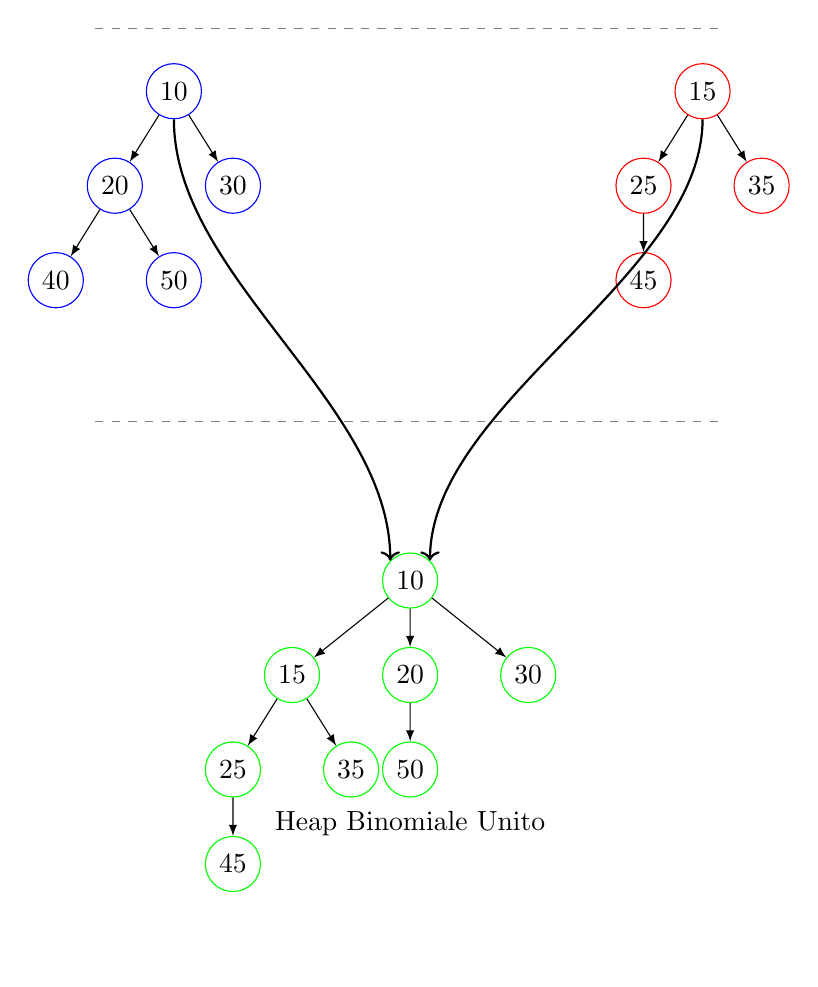
\begin{tikzpicture}[every node/.style={circle, draw, minimum size=7mm, inner sep=0pt}, 
    sibling distance=1.5cm, edge from parent/.style={draw, -latex}, level distance=1.2cm]
  
  % Primo Heap Binomiale
  \node[draw=blue] (A) {10}
      child {node[draw=blue] (B) {20}
          child {node[draw=blue] (C) {40}}
          child {node[draw=blue] (D) {50}}
      }
      child {node[draw=blue] (E) {30}};
  
  % Secondo Heap Binomiale
  \node[draw=red, right=6cm of A] (F) {15}
      child {node[draw=red] (G) {25}
          child {node[draw=red] (H) {45}}
      }
      child {node[draw=red] (I) {35}};
  
  % Heap Unito
  \node[draw=green, below=5.5cm of A, xshift=3cm] (J) {10}
      child {node[draw=green] (K) {15}
          child {node[draw=green] (L) {25}
              child {node[draw=green] (M) {45}}
          }
          child {node[draw=green] (N) {35}}
      }
      child {node[draw=green] (O) {20}
          child {node[draw=green] (Q) {50}}
      }
      child {node[draw=green] (R) {30}};
  \node[draw=none, below=1cm of J] {Heap Binomiale Unito};
  
  % Linee orizzontali per radici
  \draw[dashed, gray] (-1,0.8) -- (7,0.8);
  \draw[dashed, gray] (-1,-4.2) -- (7,-4.2);
  
  % Frecce di fusione
  \draw[->, thick] (A.south) .. controls +(down:2cm) and +(up:2cm) .. (J.north west);
  \draw[->, thick] (F.south) .. controls +(down:2cm) and +(up:2cm) .. (J.north east);
  
  \end{tikzpicture}
\end{figure}


Massimo di iterazione massimo $O(\log n)$ e quindi la complessità è $O(\log n)$.
\\
L'inserimento di un nodo non è altro che l'unione di un nodo di dimensione $0$ con l'heap binomiale a cui vogliamo aggiungere il nodo.

\subsubsection{Rimozione di un nodo}
La rimozione di un nodo in uno heap binomiale è un'operazione che può essere eseguita in tempo 
$O(logn)$. Supponendo di voler rimuovere il nodo con la chiave più piccola (che corrisponde sempre alla radice dell'heap), il processo si articola nei seguenti passi:

\begin{itemize}
  \item Identificazione della radice con chiave minima:
La radice con chiave minima può essere trovata scorrendo l'elenco delle radici degli alberi binomiali. Questo richiede tempo 

$O(logn)$, dato che il numero massimo di alberi binomiali in uno heap è proporzionale a 
logn.

\item Rimozione della radice:
Una volta identificata la radice minima, essa viene rimossa. A seguito della rimozione, i sottoalberi figli della radice vengono "scompattati". Ciascuno di questi sottoalberi è un albero binomiale separato, che può essere gestito individualmente.

\item Ricostruzione dello heap:
Per ripristinare la struttura dello heap binomiale, i sottoalberi risultanti vengono uniti tra loro e con il resto dello heap. L'operazione di unione avviene combinando alberi di gradi uguali, procedendo come nell'algoritmo di fusione. Anche questa operazione richiede 
$O(logn)$.

\end{itemize}
In sintesi, l'operazione di rimozione implica un'iterazione sugli alberi binomiali (per identificare la radice minima), seguita dalla fusione dei sottoalberi generati. Entrambe le fasi hanno complessità 
$O(logn)$, rendendo l'intero processo efficiente.



\subsubsection{Diminuzione di una chiave e rimozione di un elemento arbitrario}

Per diminuire la chiave di un nodo in uno heap binomiale, è necessario prestare attenzione a non violare la proprietà di heap. Se la chiave diminuita è minore della chiave del padre, occorre scambiare il nodo con il padre e ripetere questa operazione (nota come \textit{risalita}) fino a quando la proprietà di heap non è più violata. La complessità di questa operazione è \( O(\log n) \), poiché la profondità massima di un albero binomiale è \( O(\log n) \).
\\
La diminuzione della chiave è utile in molte applicazioni, come negli algoritmi di ottimizzazione. Tuttavia, ci sono operazioni più potenti che potrebbero comportare una complessità maggiore.
\\
Per \textbf{rimuovere un nodo arbitrario}, possiamo sfruttare l'operazione di diminuzione della chiave. Riducendo la chiave del nodo a \(-\infty\), il nodo verrà spinto alla radice, rendendo la sua rimozione equivalente a quella della radice, che richiede \( O(\log n) \) tempo.
\\
Quindi, con uno heap binomiale, è possibile eseguire le seguenti operazioni in tempo \( O(\log n) \):

\begin{itemize}
  \item Inserire un nodo
  \item Trovare il minimo
  \item Unire due heap binomiali
  \item Rimuovere la radice
  \item Diminuire una chiave
  \item Rimuovere un nodo arbitrario
\end{itemize}

Tuttavia, alcune operazioni non possono essere eseguite in tempo \( O(\log n) \):

\begin{itemize}
  \item Trovare il massimo
  \item Cercare un elemento arbitrario
\end{itemize}


\subsubsection{Trovare il mediano}

Poiché l'array di partenza non è ordinato, trovare il mediano richiede generalmente un'operazione di tempo lineare, ovvero \(O(n)\). Tuttavia, è possibile ottimizzare questo processo trasformando l'array in un heap binomiale. L'heap binomiale, sebbene non permetta l'accesso diretto al mediano, offre una struttura che può facilitare il processo.
\\
Per trovare il mediano utilizzando un heap binomiale, è necessario seguire alcuni passaggi aggiuntivi. In particolare, dopo aver costruito l'heap binomiale, si può procedere ad estrarre gli elementi in ordine crescente (o decrescente), fino a raggiungere l'elemento centrale. Sebbene l'heap binomiale non fornisca un accesso diretto alla posizione del mediano, l'ordinamento parziale che essa garantisce può ridurre il numero di operazioni necessarie rispetto a un ordinamento completo dell'array.
\\
In alternativa, un approccio come l'algoritmo di selezione del k-esimo elemento potrebbe essere utilizzato in combinazione con l'heap binomiale per trovare il mediano in modo più efficiente. 

\subsubsection{RB-Alberi e Euristiche}

Se in un RB-Albero non dobbiamo cercare la chiave precisa ma la chiave più vicina dobbiamo cercare di utilizzare l'RB Albero
in modo tale da poter usare la potenza del suo ordinamento.
Come chiave di ordinamento uso la chiave x-k ovvera la differenza tra le due misure.

\begin{lstlisting}[language = Scala]
// Primo candidato
// k valore a cui voglio avvicinarmi
// BestCandidate e' un ulteriore candidato
searchClosest(x,k) 
  if x == null
      return null
  else if(key[x] > k)
      bestCandidate = searchClosest(right[x], k)
  else if (key[x] < k)
      bestCandidate = searchClosest(left[x], k)

  if bestCandidate == null ||  (key[x] - k) < (bestCandidate - k) 
    return x
  else 
    return bestCandidate
\end{lstlisting}
Questo algoritmo ha complessità $O(\log n)$ poiché dobbiamo comunque passare per il cammino radice foglia.

\begin{examplebox}{Esempio}
Ora immaginiamo questo problema: Siamo dei venditori di macchine e conteniamo i dati delle macchine all'interno 
di un record dove sono contenuti informazioni come: prezzo di vendita, data di vendita, ecc. Vogliamo trovare la somma dei prezzi delle macchine che abbiamo venduti fino ad una certa data.
Per costruire questo tipo di albero possiamo servirci della possibilità di aggiungere campi aggiuntivi mantenibili in tempo logaritmico.
\begin{lstlisting}[language = Scala]
SearchDate(x, k)
  if(x == null) 
    return null
  else if (date[x] <= k) 
    bestDate = SearchDate(right[x], k)
    return best ?? x //equivalente a scrivere -> best != null ? best : x
  else if (date[x] > k) 
    bestDate = SearchDate(left[x], k)
    return best ?? x
\end{lstlisting}
Quindi ora abbiamo trovato il candidato migliore della data a cui possiamo applicare il rango per trovare la somma dei prezzi delle macchine vendute fino a quella data.

\end{examplebox}

\end{document}